% ============================================================================
%  PhD Pre-Synopsis Presentation
%  Title: Learning and Decision-Making in Strategic Environments
%  Author: Manish Kumar Singh | IIT Bombay | Centre for Systems and Control
%  Supervisor: Prof. Ankur A. Kulkarni
% ============================================================================
\pdfminorversion=7
\documentclass[aspectratio=169, 11pt, t, xcolor=table]{beamer}

% ── Packages ──────────────────────────────────────────────────────────────────
\usepackage{amsmath, amssymb, amsthm, mathtools}
\usepackage{centernot}
\usepackage{bbm}
\usepackage{tikz}
\usetikzlibrary{arrows.meta, positioning, calc, decorations.pathreplacing, shapes.geometric}
\usepackage{pgfplots}
\pgfplotsset{compat=1.18}
\usepackage[noend]{algpseudocode}
\usepackage{algorithm}
\usepackage{graphicx}
\usepackage{booktabs}
\usepackage{array}
\usepackage{hyperref}
\usepackage{appendixnumberbeamer}

% ── Theme & Colors ────────────────────────────────────────────────────────────
\usetheme{Madrid}
\definecolor{IITBNavy}{RGB}{0, 51, 102}
\definecolor{IITBGold}{RGB}{184, 143, 30}
\definecolor{IITBLight}{RGB}{230, 238, 248}
\definecolor{DarkRed}{RGB}{180, 30, 30}

\setbeamercolor{structure}{fg=IITBNavy}
\setbeamercolor{palette primary}{bg=IITBNavy, fg=white}
\setbeamercolor{palette secondary}{bg=IITBNavy!85, fg=white}
\setbeamercolor{palette tertiary}{bg=IITBGold, fg=white}
\setbeamercolor{frametitle}{fg=white, bg=IITBNavy}
\setbeamercolor{block title}{bg=IITBNavy!90, fg=white}
\setbeamercolor{block body}{bg=IITBLight}
\setbeamercolor{block title alerted}{bg=IITBGold!85, fg=white}
\setbeamercolor{block body alerted}{bg=IITBGold!8}
\setbeamercolor{block title example}{bg=green!55!black, fg=white}
\setbeamercolor{block body example}{bg=green!5}
\setbeamertemplate{navigation symbols}{}
\setbeamertemplate{footline}{%
  \leavevmode\hbox{%
    \begin{beamercolorbox}[wd=.30\paperwidth,ht=2.25ex,dp=1ex,center]{author in head/foot}%
      \usebeamerfont{author in head/foot}\insertshortauthor
    \end{beamercolorbox}%
    \begin{beamercolorbox}[wd=.45\paperwidth,ht=2.25ex,dp=1ex,center]{title in head/foot}%
      \usebeamerfont{title in head/foot}\insertshorttitle
    \end{beamercolorbox}%
    \begin{beamercolorbox}[wd=.25\paperwidth,ht=2.25ex,dp=1ex,right]{date in head/foot}%
      \usebeamerfont{date in head/foot}\insertframenumber{} / \inserttotalframenumber\hspace*{2ex}
    \end{beamercolorbox}%
  }\vskip0pt%
}
\setbeamerfont{frametitle}{size=\large}
\setbeamertemplate{blocks}[default]
\setbeamertemplate{itemize items}[circle]
\setbeamersize{text margin left=7mm,text margin right=7mm}
\setlength{\emergencystretch}{2em}

% Section divider slides
\AtBeginSection[]{%
  \begin{frame}[c]
    \vfill
    \centering
    \begin{beamercolorbox}[sep=10pt,center,rounded=false,shadow=false]{palette primary}
      \usebeamerfont{title}\insertsectionhead\par
    \end{beamercolorbox}
    \vfill
  \end{frame}
}

% ── Macros (from thesis) ──────────────────────────────────────────────────────
\newcommand{\E}{\mathbb{E}}
\newcommand{\prob}{\mathbb{P}}
\newcommand{\R}{\mathbb{R}}
\newcommand{\cg}[1]{\mathcal{#1}}
\newcommand{\fk}[1]{\mathfrak{#1}}
\newcommand{\msf}[1]{\mathsf{#1}}
\newcommand{\sr}[1]{\mathscr{#1}}
\newcommand{\eps}{\epsilon}
\newcommand{\dlt}{\delta}
\newcommand{\bigO}{\mathcal{O}}
\renewcommand{\H}{\mathbf{h}} % class boundary
\newcommand{\hh}{\mathbf{h}}
\newcommand{\um}{\mathbf{u_-}}
\newcommand{\up}{\mathbf{u_+}}
\newcommand{\uu}{\mathbf{u}}
\newcommand{\hminus}{\mathbf{h^{-}}}
\newcommand{\hplus}{\mathbf{h^{+}}}
\newcommand{\minus}{\mathbf{-}}
\newcommand{\plus}{\mathbf{+}}
\newcommand{\ibb}{\mathbf{i}}
\newcommand{\jbb}{\mathbf{j}}
\newcommand{\kbb}{\mathbf{k}}
\newcommand{\lbb}{\mathbf{l}}
\newcommand{\rs}{r^{\star}}
\newcommand{\srs}{s_{r^{\star}}}
\newcommand{\senpayoff}{\mathbb{U}}
% Ch3
\newcommand{\ws}{w^\star}
\newcommand{\wsz}{w^\star_z}
\newcommand{\whl}{\hat{w}_\lambda}
\newcommand{\whlc}{\hat{w}_{\lambda,c}}
\newcommand{\whlx}{\hat{w}_{\lambda,x}}
\newcommand{\whlz}{\hat{w}_{\lambda,z}}
\newcommand{\wsl}{w^\star_{\ph,\lambda}}
\newcommand{\ph}{\hat{\phi}}
\newcommand{\ps}{\phi^\star}
\newcommand{\us}{u^\star}
\newcommand{\uh}{\hat{u}}
\newcommand{\vs}{v^\star}
\newcommand{\lamz}{\lambda_z}
% Ch4
\newcommand{\RV}{R_{\mathrm{V}}}
\newcommand{\RS}{R_{\mathrm{S}}}
\newcommand{\RhatV}{\widehat{R}_{\mathrm{V}}}
\newcommand{\RhatS}{\widehat{R}_{\mathrm{S}}}
\newcommand{\I}[1]{\mathbb{I}\{#1\}}
\newcommand{\env}{\mathcal{E}}
\newcommand{\cO}{\mathcal{O}}
\newcommand{\ip}[2]{\langle #1, #2 \rangle}
\newcommand{\bV}{b_{\mathrm{V}}}

% ── Title Info ────────────────────────────────────────────────────────────────
\title[Learning in Strategic Environments]{%
  Learning and Decision-Making in\\Strategic Environments}
\subtitle{Pre-Synopsis / Defense Seminar}
\author[M.~K.~Singh]{%
  Manish Kumar Singh\\[0.1em]
  {\small Roll No.: 204230004}\\[0.2em]
  {\footnotesize Supervisor: \textbf{Prof.\ Ankur A.\ Kulkarni}}}
\institute[IIT Bombay]{%
  Centre for Systems and Control\\
  Indian Institute of Technology Bombay}
\date{2026}
\titlegraphic{
\includegraphics[height=0.85cm]{../logo-eps-converted-to.pdf}}

% ══════════════════════════════════════════════════════════════════════════════
\begin{document}
% ══════════════════════════════════════════════════════════════════════════════

% ── TITLE SLIDE ───────────────────────────────────────────────────────────────
{
\setbeamertemplate{footline}{}
\begin{frame}[c]
  \titlepage
\end{frame}
}

% ── OUTLINE ───────────────────────────────────────────────────────────────────
\begin{frame}{Outline}
  \tableofcontents
\end{frame}

% ══════════════════════════════════════════════════════════════════════════════
\section{Introduction}
% ══════════════════════════════════════════════════════════════════════════════

% ── SLIDE: Beyond Classical Learning ──────────────────────────────────────────
\begin{frame}{Beyond Classical Statistical Learning}
\small
\textbf{Central Question}\par
How should a learner act when agents respond strategically to its decisions, or when data is partitioned across non-communicating institutions?
\par\vspace{1em}
\begin{columns}[T,onlytextwidth]
\begin{column}{.47\textwidth}
\textcolor{IITBNavy}{\textbf{Strategic Behavior}}
\begin{itemize}
\item Agents manipulate features, withhold information, or alter presentation to obtain preferred decisions.
\item The deployed rule actively shapes what the learner observes.
\item Requires game-theoretic modeling of the interaction between learner and agents.
\end{itemize}
\end{column}
\begin{column}{.47\textwidth}
\textcolor{IITBNavy}{\textbf{Partitioned Observations}}
\begin{itemize}
\item Separate institutions observe $(X,Y)$ and $(X,Z)$ independently.
\item The dependence between target $Y$ and auxiliary variable $Z$ is never observed jointly.
\item Requires robust imputation and regularization to balance reliance on side information.
\end{itemize}
\end{column}
\end{columns}
\end{frame}

% ── SLIDE: Two-Stage Methodology ─────────────────────────────────────────────
\begin{frame}{Two-Stage Framework: Decision \& Learning}
\small
Across all problem settings, we employ a unified two-stage methodology:
\par\vspace{0.4em}
\begin{block}{Stage 1: The Decision Problem (Known Environment)}
\footnotesize
\begin{itemize}\itemsep=2pt
\item Specify receiver, responding agent, and objectives under complete information.
\item Formulate as a Stackelberg game: receiver commits to a rule, sender best responds.
\item Characterize structural properties of optimal rules (penalty regions, probability ramps).
\end{itemize}
\end{block}

\par\vspace{0.4em}
\begin{block}{Stage 2: The Learning Problem (Unknown Environment)}
\footnotesize
\begin{itemize}\itemsep=2pt
\item The decision maker observes only finite training samples or sequential online feedback.
\item Exploit the game structure to construct data-driven algorithms and modified hypothesis classes.
\item Establish theoretical sample complexity bounds, PAC learnability, or sublinear regret.
\end{itemize}
\end{block}
\end{frame}



% ══════════════════════════════════════════════════════════════════════════════
\section{Strategic Classification}
% ══════════════════════════════════════════════════════════════════════════════

% ── SLIDE: University Admission Motivating Example ──────────────────────────
\begin{frame}{Decision Problem: Motivating Example}
\small
\textbf{Setting: University Admissions with Strategic Applicants}
\begin{itemize}\itemsep=1pt
  \item A university admits candidates to \textbf{Theoretical Physics} ($+$) and \textbf{Experimental Physics} ($-$) via a declared entrance exam.
  \item Every applicant has a \textbf{true aptitude} aligning with a \textbf{true program}.
  \item Applicants have personal \textbf{preferences} that may not match their true aptitude.
  \item Knowing the admission rule, students can \textbf{invest coaching effort} (incurring a cost) to manipulate their demonstrated score towards their preferred program.
\end{itemize}

\par\vspace{0.3em}
\begin{alertblock}{Core Decision Question}
\centering\small
\textbf{"Given that applicants strategically game their scores, how can the university design an optimal decision rule that maximizes admissions to their true programs?"}
\end{alertblock}

\par\vspace{0.2em}
{\footnotesize \textbf{Key Challenge:} The university observes demonstrated scores, not true aptitudes. Standard naive cutoffs invite heavy manipulation and high misclassification.}
\end{frame}

% ── SLIDE: Abstract Problem Structure ───────────────────────────────────────
\begin{frame}{Strategic Classification: General Problem Structure}
\small
\textbf{Abstract Game Formulation (No specific sets or cost forms assumed)}

\par\vspace{0.3em}
\begin{columns}[T,onlytextwidth]
\begin{column}{0.48\textwidth}
\textcolor{IITBNavy}{\textbf{Receiver (Leader)}}
\begin{itemize}\itemsep=1.5pt
  \footnotesize
  \item Feature space $\cg{X}$, label space $\cg{Y}$, true target $h: \cg{X} \to \cg{Y}$.
  \item Commits to rule $r: \cg{X} \to \cg{Y} \cup \{\Delta\}$, where $\Delta$ is a \textbf{penalty label} (or reject option).
  \item \textbf{Objective:} Minimize post-response error:
    \[
      \min_{r} \prob_{x \sim D}\big( r(s_r(x)) \neq h(x) \big).
    \]
\end{itemize}
\end{column}

\begin{column}{0.48\textwidth}
\textcolor{IITBNavy}{\textbf{Sender (Follower)}}
\begin{itemize}\itemsep=1.5pt
  \footnotesize
  \item True feature $x \in \cg{X}$ drawn from prior $D$.
  \item Observes $r$; reports feature $x' \in \cg{X}$ maximizing net payoff:
    \[
      s_r(x) \in \arg\max_{x' \in \cg{X}} \big[ U(r(x'), x) - C(x, x') \big].
    \]
  \item $U(\Delta, x) = -\infty$; $C(x, x) = 0$.
  \item Ties broken in worst case against receiver.
\end{itemize}
\end{column}
\end{columns}

\par\vspace{0.4em}
\begin{block}{Stackelberg Equilibrium Concept}
\footnotesize
A Stackelberg equilibrium rule $\rs$ anticipates the follower's worst-case best response $s_r(x)$ and optimizes receiver classification accuracy over all commitments $r \in \msf{R}$.
\end{block}
\end{frame}

% ── SLIDE: Discrete Problem Formulation ─────────────────────────────────────
\begin{frame}{Discrete Decision Problem: Formulation}
\small
\textbf{Specifics of the Discrete Setting}
\begin{itemize}\itemsep=2pt
  \item \textbf{Feature Space:} A finite set $\cg{X} = \{1, 2, \ldots, n\}$.
  \item \textbf{True Function:} $h: \cg{X} \to \cg{Y} = \{\minus, \plus\}$ partitions points into two classes.
  \item \textbf{Sender Utility:} Normalized such that getting the true label yields zero utility:
    $U(h(x), x) = 0$, $U(\Delta, x) = -\infty$, and $U(y, x) \ge 0$ for $y \ne h(x)$.
  \item \textbf{Manipulation Cost:} General cost matrix $C: \cg{X} \times \cg{X} \to \R_{\ge 0}$ with $C(x,x) = 0$.
  \item \textbf{Receiver Strategy:} Deterministic assignment $r: \cg{X} \to \{\minus, \plus, \Delta\}$.
\end{itemize}

\par\vspace{0.4em}
\begin{alertblock}{The Strategic Conflict on Discrete Domains}
\footnotesize
An agent of true type $\ibb$ ($h(\ibb) = \minus$) will impersonate report $\lbb$ intended for type $\jbb$ ($h(\jbb) = \plus$) whenever the utility gain exceeds the cost difference:
\[
  U(h(\jbb), \ibb) - C(\lbb, \ibb) + C(\kbb, \ibb) \ge 0.
\]
\textbf{Goal:} Identify which points can be safely classified and which must receive penalty label $\Delta$.
\end{alertblock}
\end{frame}

% ── SLIDE: Discrete Problem Theorems ─────────────────────────────────────────
\begin{frame}{Discrete Setting: Equivalence to Maximum Independent Set}
\small
\begin{block}{Definition 2.4 (Sender's Conflict Graph $G_h$)}
\footnotesize
Let $G_h = (V,E)$ with $V = \cg{X}^2$; node $(\ibb,\kbb)$ denotes true feature $\ibb$ reporting $\kbb$.
Nodes $(\ibb,\kbb)$ and $(\jbb,\lbb)$ have an undirected edge iff:
\begin{enumerate}\itemsep=0pt
  \item[(a)] $\ibb = \jbb, \kbb \neq \lbb$ (unique reporting), or $h(\ibb) \neq h(\jbb), \kbb = \lbb$ (label clash);
  \item[(b)] $h(\ibb) \neq h(\jbb)$ and manipulation incentive holds:
  $U(h(\jbb),\ibb) - C(\lbb,\ibb) + C(\kbb,\ibb) \geq 0$ (or vice versa).
\end{enumerate}
\end{block}
\vspace{0.1em}
\begin{block}{Theorem 2.5 (Stackelberg Equilibrium $\Longleftrightarrow$ Maximum Independent Set)}
\footnotesize
\begin{itemize}\itemsep=0pt
  \item[(a)] If $I^\star$ is a \textbf{maximum independent set} (MIS) of $G_h$, then
  $\rs(\kbb; I^\star) = h(\ibb)$ if $\exists \ibb \text{ s.t. } (\ibb,\kbb) \in I^\star$, and $\Delta$ otherwise,
  is a Stackelberg equilibrium.
  \item[(b)] Conversely, any Stackelberg equilibrium $\rs$ defines an MIS with $|I^\star| = \alpha(G_h)$.
\end{itemize}
\end{block}
\vspace{0.1em}
\begin{alertblock}{Combinatorial Takeaway}
\footnotesize
Optimal discrete classification reduces to finding an MIS on $G_h$; points not in the MIS receive penalty $\Delta$.
\end{alertblock}
\end{frame}

% ── SLIDE: Discrete Example and Graph Application ───────────────────────────
\begin{frame}{Discrete Setting: Application \& Graph Construction}
\small
\begin{columns}[T,onlytextwidth]
\begin{column}{0.50\textwidth}
\textbf{Illustrative 3-Point Setup \& Conflict Graph:}
\begin{itemize}\itemsep=0.5pt
  \footnotesize
  \item $\cg{X} = \{1, 2, 3\}$, with $h(1)=h(2)=\minus$ and $h(3)=\plus$.
  \item Cost $C(i, j) = |i - j|$; utility $U(\plus, 2) = 1.5$.
  \item Type $2$ games: $U(\plus, 2) - C(3,2) = 0.5 > 0$.
  \item Node $(2,2)$ conflicts with $(3,3)$ via gaming edge.
  \item MIS is $I^\star = \{(1,1), (3,3)\}$ ($\alpha(G_h) = 2$).
  \item \textbf{Optimal Rule:} $r(1) = \minus,\; r(3) = \plus,\; \mathbf{r(2) = \Delta}$.
\end{itemize}

\vspace{0.1em}
\begin{alertblock}{Contrast: Naive vs.\ Strategic Rule}
\scriptsize
\textbf{Naive rule $h$ (no $\Delta$):} Type $2$ flips to $3 \implies$ \textbf{Loss = 1}.\\
\textbf{Strategic rule $\rs$:} $r(2) = \Delta$ deters gaming $\implies$ \textbf{Loss = 0} on $\{1, 3\}$!
\end{alertblock}
\end{column}

\begin{column}{0.48\textwidth}
\centering
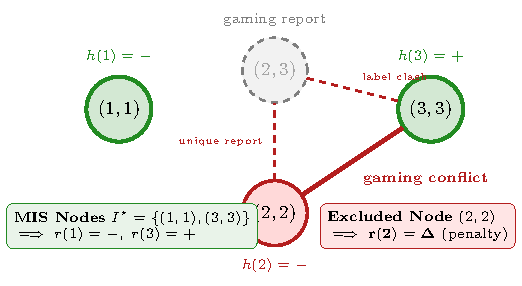
\includegraphics[width=\linewidth,height=3.1cm,keepaspectratio]{reviewed_assets/discrete_conflict_graph.pdf}
\par{\scriptsize Conflict graph $G_h$ for 3-point domain (Thesis Sec.\ 2.3.1)}
\end{column}
\end{columns}
\end{frame}

% ── SLIDE: Continuous 1D Problem Formulation ────────────────────────────────
\begin{frame}{Continuous 1D Decision Problem: Specific Formulation}
\small
\textbf{Specifics of the Continuous 1D Setting}
\begin{itemize}\itemsep=1.5pt
  \item \textbf{Domain:} $\cg{X} = [0, 1]$, continuous distribution $D$ with density $f_D(x) > 0$.
  \item \textbf{True Classifier:} Threshold classifier with class boundary $\hh \in (0, 1)$:
    \[
      h(x) = \begin{cases} \minus & x \in [0, \hh], \\ \plus & x \in (\hh, 1]. \end{cases}
    \]
  \item \textbf{Non-Uniform Preferences:} Senders have label-switching utilities:
    $U(\plus, x) = \up$ ($x \le \hh$), $U(\minus, x) = \um$ ($x > \hh$), $U(\Delta, x) = -\infty$.
  \item \textbf{Manipulation Cost:} Cost kernel $C(x, x') = |\phi(x') - \phi(x)|$, $\phi$ strictly increasing.
\end{itemize}

\par\vspace{0.3em}
\textbf{Regimes of Strategic Behavior:}
\begin{itemize}\itemsep=1.5pt
  \item \textbf{Cases 1--3 (Trivial):} Aligned preferences ($\up, \um \le 0$) or manipulation too cheap ($\up \ge 1$) $\implies$ truthful or trivial majority rule.
  \item \textbf{Cases 4 \& 5 (Strategic Regimes):} $0 < \up \le 1$ and $\um \le \up$.
    Manipulation is actively controlled by deploying the \textbf{penalty label $\Delta$}.
\end{itemize}
\end{frame}

% ── SLIDE: Continuous 1D Problem Theorems ───────────────────────────────────
\begin{frame}{Continuous 1D Setting: Deterministic Stackelberg Theorems}
\small
\begin{block}{Theorem 2.10 (Deterministic Stackelberg Equilibrium — Case 4)}
\footnotesize
Let $0 < \up \le 1$ and $-\up < \um \le \up$. Define cutoffs $\hminus, \hplus$ such that $0 \le \hminus \le \hh < \hplus \le 1$ and $\phi(\hplus) - \phi(\hminus) = \up$. Then the receiver strategy
\[
  r(x;\hminus,\hplus) = \begin{cases}
    h(x) & x \in [0,\hminus] \cup [\hplus, 1], \\
    \Delta & x \in (\hminus, \hplus),
  \end{cases}
\]
is a Stackelberg equilibrium. The optimal pair $(\hminus,\hplus)$ minimizes the mass $D((\hminus,\hplus))$.
\end{block}

\par\vspace{0.2em}
\begin{block}{Theorem 2.11 (Case 5: Zero Classification Error!)}
\footnotesize
When sender preferences are strongly opposing ($1 \ge \up > 0$ and $\um \le -\up$), setting $\hminus = \hh$ and $\phi(\hplus) - \phi(\hh) = \up$ achieves \textbf{Zero Classification Error}:
$\cg{E}(\rs) = \mathbf{0}$.
\end{block}

\par\vspace{0.2em}
\footnotesize
\textbf{Mechanism:} Receiver creates a \emph{buffer zone} of width $\up$ around the boundary. The penalty region deters crossing and strictly confines misclassification.
\end{frame}

% ── SLIDE: Continuous Example & Naive vs Strategic Comparison ───────────────
\begin{frame}{Continuous Setting: Example \& Naive vs.\ Strategic Gain}
\small
\textbf{Canonical Setting:} Uniform $D$ on $[0,1]$, $\phi(x) = x$, boundary $\hh = 0.5$, symmetric utility $2\uu$.

\par\vspace{0.2em}
\begin{columns}[T,onlytextwidth]
\begin{column}{0.48\textwidth}
\textcolor{DarkRed}{\textbf{1. Naive Rule $h(x)$ (Passive)}}
\begin{itemize}\itemsep=1pt
  \footnotesize
  \item Boundary placed at $\hh=0.5$.
  \item Senders in $(\hh-2\uu, \hh]$ flip to $\plus$; senders in $(\hh, \hh+2\uu]$ flip to $\minus$.
  \item Misclassification over $(\hh-2\uu, \hh+2\uu]$:
    $\mathbf{\cg{E}(h) = 4\uu}$.
\end{itemize}
\centering
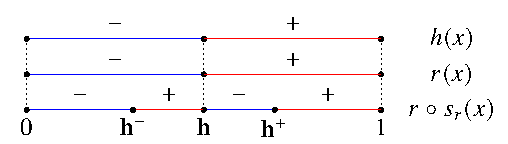
\includegraphics[width=\linewidth,height=1.1cm,keepaspectratio]{reviewed_assets/ch2_naive.pdf}
\end{column}

\begin{column}{0.48\textwidth}
\textcolor{IITBNavy}{\textbf{2. Strategic Rule $\rs$ (With Penalty $\Delta$)}}
\begin{itemize}\itemsep=1pt
  \footnotesize
  \item Sets buffer $(\hh-\uu, \hh+\uu)$ to $\Delta$.
  \item Penalty $-\infty$ prevents cross-boundary gaming.
  \item Misclassification strictly $[\hh-\uu, \hh+\uu]$:
    $\mathbf{\cg{E}(\rs) = 2\uu \quad \text{(50\% Reduction!)}}$
\end{itemize}
\centering
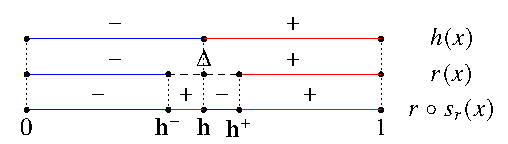
\includegraphics[width=\linewidth,height=1.1cm,keepaspectratio]{reviewed_assets/ch2_deterministic.pdf}
\end{column}
\end{columns}

\par\vspace{0.3em}
\begin{alertblock}{University Admission Interpretation}
\footnotesize
Excluding boundary questions (difficulty in $[0.48, 0.52]$) prevents borderline candidates from gaming programs, cutting misclassification error strictly in half.
\end{alertblock}
\end{frame}

% ── SLIDE: Multi-Dimensional Generalization ─────────────────────────────────
\begin{frame}{Continuous Setting: Multi-Dimensional Generalization}
\small
\textbf{Higher Dimensions: Linear Boundary in $\R^n$ (Thesis Sec.\ 2.3.3)}
\begin{itemize}\itemsep=0.5pt
  \footnotesize
  \item Feature space $\cg{X} \subset \R^n$ (bounded convex set, uniform $D$). Cost: $\|x - x'\|_2$.
  \item Ground truth: Hyperplane boundary $h(x) = \plus$ if $w^\top x > \hh$, else $\minus$ (unit normal $w \in \R^n$).
  \item Boundary surface set $\cg{Z} = \{z \in \cg{X} : w^\top z = \hh\}$ with normalized area $\sigma(\cg{Z}) = \frac{\mathcal{H}^{n-1}(\cg{Z})}{\text{Vol}(\cg{X})}$.
\end{itemize}

\vspace{0.05em}
\begin{block}{Theorems 2.12 \& 2.13 (The Optimal $\Delta$-Slab Equilibrium)}
\footnotesize
\begin{itemize}\itemsep=0.5pt
  \item \textbf{Lower Bound:} For \emph{any} deterministic receiver rule $r$, $\cg{E}(r) \ge 2\uu \cdot \sigma(\cg{Z})$.
  \item \textbf{Optimal $\Delta$-Slab Strategy:} Parallel slab of width $2\uu$ with penalty label $\Delta$:
  \begin{center}
  \vspace{-0.4em}
  $\rs(x) = \plus \text{ if } w^\top x \ge \hh+\uu; \quad \minus \text{ if } w^\top x \le \hh-\uu; \quad \Delta \text{ if } |w^\top x - \hh| < \uu,$
  \vspace{-0.4em}
  \end{center}
  achieving the lower bound with \textbf{exact equality}: $\cg{E}(\rs) = \mathbf{2\uu \cdot \sigma(\cg{Z})}$.
\end{itemize}
\end{block}

\vspace{0.05em}
\begin{alertblock}{Equivalence via Dimension Reduction}
\scriptsize
The scalar projection mapping $\cg{M}(x) = \frac{w^\top x - a_{\min}}{a_{\max} - a_{\min}}$ projects $\R^n \to [0,1]$, proving that 1D structural properties and buffer geometry generalize directly to multi-dimensional linear classifications!
\end{alertblock}
\end{frame}

% ── SLIDE: Stochastic Problem Formulation & Theorem ─────────────────────────
\begin{frame}{Stochastic Decision Problem: Formulation \& Theorem}
\small
\textbf{Specifics of the Stochastic Formulation}
\begin{itemize}\itemsep=1.5pt
  \item Receiver strategy is randomized: $r(x) = \big(p(x), q(x), \delta(x)\big) \in \Delta(\{\minus, \plus, \Delta\})$.
  \item Sender chooses report $x'$ to maximize expected payoff:
    \[
      s_r(x) \in \arg\max_{x' \in [0,1]} \Big[ \E_{y \sim r(x')}[U(y, x)] - |\phi(x') - \phi(x)| \Big].
    \]
\end{itemize}

\par\vspace{0.3em}
\begin{block}{Theorem 2.14 (Stochastic Stackelberg Equilibrium)}
\footnotesize
Let $D$ be uniform on $[0,1]$, $\phi(x) = x$, $\up = \um = 2\uu$, and define $\hminus = \hh - \uu$, $\hplus = \hh + \uu$.
The randomized decision rule with \textbf{no penalty label} ($\delta(x) \equiv 0$):
\[
  \rs(x) = \begin{cases}
    (1,\, 0,\, 0) & x \le \hminus, \\
    \left(1 - \frac{x-\hminus}{2\uu},\, \frac{x-\hminus}{2\uu},\, 0\right) & x \in (\hminus, \hplus), \\
    (0,\, 1,\, 0) & x \ge \hplus,
  \end{cases}
\]
is a Stackelberg equilibrium achieving expected error $\cg{E}(\rs) = \frac{\uu}{2}$.
\end{block}
\end{frame}

% ── SLIDE: Stochastic Interpretation and Error Comparison ───────────────────
\begin{frame}{Stochastic Setting: Interpretation \& Three-Way Comparison}
\small
\begin{columns}[T,onlytextwidth]
\begin{column}{0.54\textwidth}
\textbf{Mechanism: Why Randomization Works}
\begin{itemize}\itemsep=1pt
  \footnotesize
  \item Probability $q(x)$ ramps linearly with slope $\frac{1}{2\uu}$.
  \item Marginal utility gain: $2\uu \times \frac{1}{2\uu} = 1$.
  \item Matches marginal cost of effort $\frac{\partial}{\partial x'} |x'-x| = 1$!
  \item Marginal gain matches cost everywhere $\implies$ truth-telling $s_r(x) = x$ is optimal!
\end{itemize}
\end{column}

\begin{column}{0.44\textwidth}
\centering
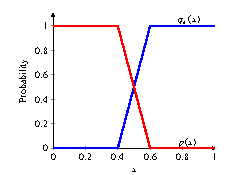
\includegraphics[width=\linewidth,height=2.0cm,keepaspectratio]{reviewed_assets/ch2_stochastic.pdf}
\par{\scriptsize Linear ramp $q(x)$ and $p(x)$ (Thesis Fig.\ 2.3)}
\end{column}
\end{columns}

\par\vspace{0.3em}
\renewcommand{\arraystretch}{1.1}
\centering
\footnotesize
\begin{tabular}{@{}lccc@{}}
\toprule
& \textbf{Naive Rule} & \textbf{Deterministic $\Delta$-Rule} & \textbf{Stochastic Ramp Rule} \\
\midrule
\textbf{Receiver Error} & $\mathbf{4\uu}$ & $\mathbf{2\uu}$ & $\mathbf{\uu/2}$ \\
\textbf{Relative Gain} & Baseline ($0\%$) & \textbf{50\% reduction} & \textbf{87.5\% reduction!} \\
\textbf{Mechanism} & Passive & Buffer region with $\Delta$ & Continuous probability ramp \\
\bottomrule
\end{tabular}

\par\vspace{0.2em}
\raggedright
\scriptsize
\textbf{Insight:} Randomization provides continuous leverage. The penalty label $\Delta$ compensates for the absence of randomization when deterministic rules are legally or practically required.
\end{frame}

% ── SLIDE: Fairness and Complexity Trade-off ────────────────────────────────
\begin{frame}{Decision Problem: Fairness vs.\ Complexity Trade-off}
\small
\textbf{Equilibrium Multiplicity in Deterministic Rules:}\\
{\footnotesize Any interval $[\hminus, \hplus]$ of length $2\uu$ containing $\hh = 0.5$ achieves minimal error $2\uu$, but structures differ:}
\vspace{0.1em}
\begin{columns}[T,onlytextwidth]
\begin{column}{0.48\textwidth}
\textbf{Rule 1 (Symmetric Buffer $[0.45, 0.55]$):}
\begin{itemize}\itemsep=0pt
  \footnotesize
  \item Equal errors on both classes $\implies$ \textbf{Fair}.
  \item Induced classifier $r_1 \circ s_{r_1}$ has \textbf{3 boundaries} $\implies$ higher VC dimension!
\end{itemize}
\vspace{0.1em}
\textbf{Rule 2 (Asymmetric Buffer $[0.40, 0.50]$):}
\begin{itemize}\itemsep=0pt
  \footnotesize
  \item Errors only on class $\minus$ $\implies$ \textbf{Unfair}.
  \item Induced classifier $r_2 \circ s_{r_2}$ has \textbf{2 boundaries} $\implies$ lower VC dimension!
\end{itemize}
\end{column}
\begin{column}{0.48\textwidth}
\centering
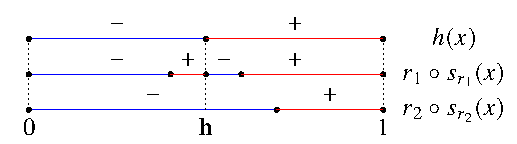
\includegraphics[width=\linewidth,height=1.35cm,keepaspectratio]{reviewed_assets/ch2_fairness.pdf}
\par{\scriptsize Thesis Fig.\ 2.4: Induced boundaries under $r_1$ vs $r_2$}
\end{column}
\end{columns}
\vspace{0.1em}
\begin{alertblock}{Fundamental Trade-off}
\footnotesize
Enforcing \textbf{group fairness} increases the boundary complexity (VC dimension), requiring higher sample complexity to learn!
\end{alertblock}
\end{frame}

% ── SLIDE: Sender Participation Constraints ─────────────────────────────────
\begin{frame}{Decision Problem: Sender Participation Constraints}
\small
\textbf{The Principal-Agent Perspective: Preventing Degenerate Rules}
\begin{itemize}\itemsep=0.5pt
  \item Minimizing error without constraints could lead to degenerate rules (e.g., $r(x) = \Delta$ a.e.).
  \item Senders in practice have an outside \textbf{reservation payoff} $\nu$.
\end{itemize}
\vspace{0.15em}
\begin{columns}[T,onlytextwidth]
\begin{column}{0.48\textwidth}
\textcolor{IITBNavy}{\textbf{Negative Reservation ($\nu \le 0$)}}
\begin{itemize}\itemsep=0.5pt
  \footnotesize
  \item Senders opt out only if suffering negative payoff.
  \item Degenerate rules yield $-\infty$ $\implies$ sender rejects.
  \item Symmetric buffer $r_1$ satisfies participation:
    $\min_{x} \mathbb{U}(x; r_1, s_{r_1}) = 0 \ge \nu$.
\end{itemize}
\end{column}
\begin{column}{0.48\textwidth}
\textcolor{IITBNavy}{\textbf{Positive Reservation ($\nu > 0$)}}
\begin{itemize}\itemsep=0.5pt
  \footnotesize
  \item Senders require a positive baseline reward.
  \item Truthful reporting yields utility $0 < \nu$, so participation constraints bind tightly across domain.
  \item Rules must balance deterrence with participation.
\end{itemize}
\end{column}
\end{columns}
\vspace{0.15em}
\begin{block}{Takeaway}
\footnotesize
Participation constraints rule out degenerate penalty assignments and provide an economic foundation for selecting non-degenerate buffer equilibria.
\end{block}
\end{frame}

% ── SLIDE: Learning Setup & Multiple Boundaries ─────────────────────────────
\begin{frame}{Strategic Learning: Motivation \& Problem Setup}
\small
\textbf{The Learning Paradigm: Unknown Environment (Thesis Sec.\ 2.4)}
\begin{itemize}\itemsep=0.5pt
  \footnotesize
  \item Receiver knows game structure ($C, U$), but not ground truth $h$ or distribution $D$.
  \item Observes finite training sample $S = \{(x_i, y_i)\}_{i=1}^m \stackrel{\text{i.i.d.}}{\sim} D$.
  \item \textbf{Strategic PAC Learnability (Def.\ 2.17):} Outputs $\hat{r}$ such that with prob $> 1-\delta$:
  \[
    \cg{E}(\hat{r}; h, D) - \cg{E}(\rs_{h,D}; h, D) < \eps \quad \text{for } m \ge m_{\cg{F}}(\eps,\dlt).
  \]
\end{itemize}

\vspace{0.1em}
\begin{block}{Multiple Decision Boundaries: Generalizing to $\text{VC}(\cg{F}) = d$}
\footnotesize
\begin{itemize}\itemsep=0.5pt
  \item \textbf{Hypothesis Class:} $\cg{F} \subset \{f: [0,1] \to \{\minus, \plus\}\}$ with at most $d-1$ decision boundaries ($\implies \mathbf{\text{VC}(\cg{F}) = d}$).
  \item \textbf{Stackelberg Structure (Prop.\ 2.16):} For intervals $O_1, \dots, O_{d-1}$, optimal rule assigns active sub-intervals $\Theta_n \subseteq O_n$ to $h(x)$ and intervening buffer zones to penalty $\Delta$.
  \item Guarantees that multi-boundary 1D problems preserve piecewise Stackelberg structure.
\end{itemize}
\end{block}
\end{frame}

% ── SLIDE: Two Strategic Learning Algorithms ────────────────────────────────
\begin{frame}{Two Strategic Learning Algorithms}
\small
\begin{columns}[T,onlytextwidth]
\begin{column}{0.48\textwidth}
\begin{block}{Algorithm 1: Vanilla ERM (Two-Stage)}
\begin{algorithmic}[1]
\footnotesize
\State \textbf{Input:} $\cg{F}$, sample $S = \{(x_i,y_i)\}_{i=1}^m$
\State \textbf{Estimation:} Fit non-strategic rule:
\[
  \hat{h} \gets \arg\min_{f \in \cg{F}} \sum_{i=1}^m \mathbbm{1}_{\{f(x_i) \neq y_i\}}
\]
\State Estimate empirical law $D(S)$
\State \textbf{Decision:} Deploy Stackelberg rule:
\[
  \hat{r} \gets \rs_{\hat{h}, D(S)} \quad \text{(plug-in)}
\]
\State \textbf{Output:} $\hat{r}$
\end{algorithmic}
\end{block}
\par{\footnotesize \textcolor{IITBNavy}{\textbf{Philosophy:}} Decouples estimation from game; ignores gaming during training.}
\end{column}

\begin{column}{0.48\textwidth}
\begin{block}{Algorithm 2: Strategy-Aware ERM (SERM)}
\begin{algorithmic}[1]
\footnotesize
\State \textbf{Input:} $\cg{F}$, sample $S = \{(x_i,y_i)\}_{i=1}^m$
\State \textbf{Transform:} Stackelberg class:
\[
  \widetilde{\cg{F}} \gets \{ \rs_{f,D} \circ s_{\rs_{f,D}} : f \in \cg{F}, D \in \fk{D} \}
\]
\State \textbf{Strategic ERM:} Optimize directly:
\[
  \hat{r} \circ s_{\hat{r}} \gets \arg\min_{\widetilde{f} \in \widetilde{\cg{F}}} \sum_{i=1}^m \mathbbm{1}_{\{\widetilde{f}(x_i) \neq y_i\}}
\]
\State \textbf{Output:} $\hat{r}$
\end{algorithmic}
\end{block}
\par{\footnotesize \textcolor{IITBNavy}{\textbf{Philosophy:}} Embeds game incentives directly into empirical risk optimization.}
\end{column}
\end{columns}
\end{frame}

% ── SLIDE: Fundamental Learning Theorems ────────────────────────────────────
\begin{frame}{Strategic Learning: Fundamental Theorems}
\small
\begin{block}{Fundamental Theorems of Strategic Learning}
\footnotesize
\begin{itemize}\itemsep=1.5pt
  \item \textbf{Theorem 2.21 (Equivalence):} Let $\cg{F}$ have $\le d-1$ boundaries. Then $\cg{F}$ is \textbf{strategically learnable under Strategy-Aware ERM} if and only if
  \[
    \mathbf{\text{VC dim}(\widetilde{\cg{F}}) < \infty}.
  \]
  \item \textbf{Corollary 2.22 (Hierarchy):} For standard $\cg{F}$ and induced Stackelberg class $\widetilde{\cg{F}}$:
  \[
    \mathbf{\text{VC dim}(\cg{F}) < \infty \implies \text{VC dim}(\widetilde{\cg{F}}) < \infty}.
  \]
  \par{\scriptsize \textbf{Implication:} Any class learnable by Vanilla ERM is also learnable by Strategy-Aware ERM.}
\end{itemize}
\end{block}

\vspace{0.1em}
\begin{block}{Sample Complexity Comparison}
\footnotesize
\begin{itemize}\itemsep=1pt
  \item \textbf{Vanilla ERM:} Sample complexity $m(\eps, \dlt) = \Theta\left(\frac{d \log(1/\eps) + \log(1/\dlt)}{\eps}\right)$ via DKW theorem.
  \item \textbf{Strategy-Aware ERM:} Sample complexity governed directly by $\widetilde{d} = \text{VC dim}(\widetilde{\cg{F}})$.
\end{itemize}
\end{block}
\end{frame}

% ── SLIDE: Complexity Punchline & Heuristics ─────────────────────────────────
\begin{frame}{Complexity Punchline: Infinite vs.\ Finite VC Dimension}
\small
\begin{alertblock}{The Asymmetry Punchline: $\text{VC}(\cg{F}) = \infty \centernot\implies \text{VC}(\widetilde{\cg{F}}) = \infty$ (Example 2.23)}
\footnotesize
\begin{itemize}\itemsep=1pt
  \item Consider rational-subset hypothesis class $f_F(x)$ where $F \subseteq ([\mathbf{f}, 1] \cap \mathbb{Q})$.
  \item Class can shatter arbitrarily large subsets of rationals $\implies \mathbf{\text{VC}(\cg{F}) = \infty}$! Vanilla ERM fails.
  \item Yet strategic penalty deterrence collapses equilibrium to constant rule $r \equiv \minus \implies \mathbf{\text{VC}(\widetilde{\cg{F}}) = 0}$!
  \item \textbf{Punchline:} Strategic incentives can compress infinite complexity into finite learnability!
\end{itemize}
\end{alertblock}

\vspace{0.15em}
\textbf{Finite-Dimensional Regime Selection (Example 2.24):}
\begin{columns}[T,onlytextwidth]
\begin{column}{0.48\textwidth}
\begin{exampleblock}{Wide Intervals ($k > 1$)}
\footnotesize
\begin{itemize}\itemsep=0.5pt
  \item Class boundaries expand to $3n$.
  \item $\text{VC}(\widetilde{\cg{F}}) \ge \text{VC}(\cg{F})$.
  \item \textbf{Recommendation:} \textbf{Vanilla ERM} is simpler and more sample-efficient.
\end{itemize}
\end{exampleblock}
\end{column}
\begin{column}{0.48\textwidth}
\begin{exampleblock}{Narrow Intervals ($k \le 1$)}
\footnotesize
\begin{itemize}\itemsep=0.5pt
  \item Minority intervals collapse to $\Delta$.
  \item Boundaries drop to $1 \ll n$.
  \item \textbf{Recommendation:} \textbf{SERM} dramatically compresses learning!
\end{itemize}
\end{exampleblock}
\end{column}
\end{columns}
\end{frame}


% ══════════════════════════════════════════════════════════════════════════════
\section{Learning with Side Information}
% ══════════════════════════════════════════════════════════════════════════════

% ── SLIDE: Ch3 Motivation & Setting ──────────────────────────────────────────
\begin{frame}{Side Information: Motivation \& Setting}
\small
\textbf{Setting: Available Test-Time Side Information from Partitioned Data}
\begin{itemize}\itemsep=1pt
  \item At test time, an auxiliary variable $Z \in \{-1, +1\}$ is available alongside features $X$ to predict $Y$.
  \item \textbf{Example:} University admissions ($Y$) aided by a secondary college decision ($Z$), or primary hospital diagnosis assisted by secondary laboratory testing.
\end{itemize}

\vspace{0.15em}
\begin{columns}[T,onlytextwidth]
\begin{column}{0.48\textwidth}
\textcolor{IITBNavy}{\textbf{Partitioned Training Data:}}\\
\small $D = \{(x_i, y_i)\}_{i=1}^n, \quad S = \{(x_j, z_j)\}_{j=1}^m$.
\begin{itemize}\itemsep=0.5pt
  \footnotesize
  \item Disjoint institutional silos.
  \item Target $Y$ and side info $Z$ are \textbf{never observed jointly}!
\end{itemize}
\end{column}

\begin{column}{0.48\textwidth}
\textcolor{IITBNavy}{\textbf{Test-Time Deployment:}}\\
\small Predict outcome $Y$ using joint $(X, Z)$.
\begin{itemize}\itemsep=0.5pt
  \footnotesize
  \item Full information $(X,Z)$ is available.
  \item Learner must bridge data partition.
\end{itemize}
\end{column}
\end{columns}

\vspace{0.05em}
\begin{alertblock}{Core Decision Question}
\footnotesize
\textbf{``How can a learner optimally exploit test-time side information $Z$ when its joint relationship with $Y$ was never observed during training?''}
\end{alertblock}
\end{frame}

% ── SLIDE: Ch3 Formulation & Imputation ──────────────────────────────────────
\begin{frame}{Partitioned Data: Formulation \& Imputation Process}
\small
$(X,Y,Z) \sim \cg{D}$ on $\cg{X} \times \{-1,1\}^2$. Regularity conditions (C1)--(C4) hold (boundedness, positive definiteness, non-separability).

\vspace{0.1em}
\textbf{Classifiers (Logistic Loss $\ell(a,b;c) = -\ln(\sigma(b \cdot c^\top(1,a)))$):}
\begin{itemize}\itemsep=0.5pt
  \footnotesize
  \item \textbf{Secondary Imputer:} $\uh \gets \arg\min_u \hat{L}(u) + \mu\|u\|^2$ on $S \implies \ph(x) = \text{sign}(\hat{u}_c + \hat{u}_x^\top x)$ maps $X \to Z$.
  \item \textbf{Target Composite:} $\whl \gets \arg\min_w \hat{R}^{\ph}(w) + \lambda_c|w_c|^2 + \lambda_x\|w_x\|^2 + \lamz|w_z|^2$ on imputed $D$.
\end{itemize}

\vspace{0.1em}
\begin{center}
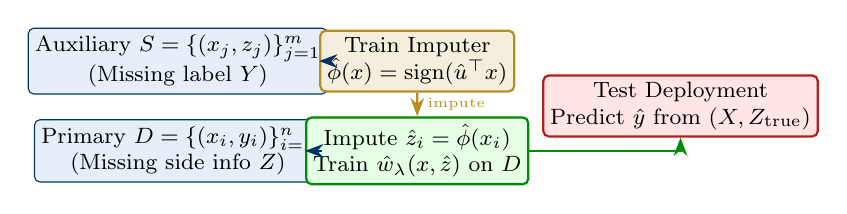
\begin{tikzpicture}[scale=0.76, font=\footnotesize, >=Stealth,
    block/.style={draw=IITBNavy, rounded corners=2pt, fill=IITBLight, align=center, inner sep=2.5pt},
    gold/.style={draw=IITBGold, thick, rounded corners=2pt, fill=IITBGold!15, align=center, inner sep=2.5pt},
    green/.style={draw=green!55!black, thick, rounded corners=2pt, fill=green!10, align=center, inner sep=2.5pt},
    red/.style={draw=DarkRed, thick, rounded corners=2pt, fill=red!10, align=center, inner sep=2.5pt}
  ]
  \node[block] (S) at (0, 0.9) {Auxiliary $S = \{(x_j, z_j)\}_{j=1}^m$\\(Missing label $Y$)};
  \node[block] (D) at (0, -0.6) {Primary $D = \{(x_i, y_i)\}_{i=1}^n$\\(Missing side info $Z$)};
  \node[gold] (imp) at (4.0, 0.9) {Train Imputer\\$\ph(x) = \text{sign}(\hat{u}^\top x)$};
  \node[green] (comp) at (4.0, -0.6) {Impute $\hat{z}_i = \ph(x_i)$\\Train $\whl(x, \hat{z})$ on $D$};
  \node[red] (test) at (8.4, 0.15) {Test Deployment\\Predict $\hat{y}$ from $(X, Z_{\text{true}})$};

  \draw[->, thick, IITBNavy] (S) -- (imp);
  \draw[->, thick, IITBGold] (imp) -- node[right, font=\tiny] {impute} (comp);
  \draw[->, thick, IITBNavy] (D) -- (comp);
  \draw[->, thick, green!55!black] (comp) -| (test);
\end{tikzpicture}
\end{center}
\end{frame}

% ── SLIDE: PSIL Algorithm ────────────────────────────────────────────────────
\begin{frame}{Partitioned Side Information Learning (PSIL)}
\begin{block}{Algorithm 3.1: Partitioned Side Information Learning (PSIL)}
\begin{algorithmic}[1]
\footnotesize
\Require Primary dataset $D = \{(x_i, y_i)\}_{i=1}^n$, auxiliary dataset $S = \{(x_j, z_j)\}_{j=1}^m$
\Ensure Composite classifier $\whl: \cg{X} \times \cg{Z} \to \cg{Y}$
\State \textbf{Step 1 (Train Imputer):} Learn $\uh = \arg\min_{u} \hat{L}(u) + \frac{c}{\sqrt{m}}\|u\|^2$ on $S$; set $\ph(x) = \text{sign}(\hat{u}_c + \hat{u}_x^\top x)$.
\State \textbf{Step 2 (Data Imputation):} For each $(x_i, y_i) \in D$, compute imputed side information $\hat{z}_i \gets \ph(x_i)$.
\State \textbf{Step 3 (Regularized Learning):} Set $\lambda_c = \lambda_x = 1/\sqrt{n}$, and choose $\lamz \ge 1/\sqrt{n}$. Compute
\[
  \whl \gets \arg\min_{w \in \R^{d+2}} \hat{R}^{\ph}(w) + \lambda_c |w_c|^2 + \lambda_x \|w_x\|^2 + \lamz |w_z|^2.
\]
\State \textbf{Step 4 (Deployment):} Given test point $(x, z)$ with observed $z$, predict $\hat{y} = \text{sign}(\whlc + \whlx^\top x + \whlz z)$.
\end{algorithmic}
\end{block}

\vspace{0.15em}
\par{\footnotesize \textbf{Crucial Role of $\lamz$:} Controls trust in imputed side information. Tuning $\lamz$ balances exploiting $Z$'s predictive signal against protecting against imputation error in $\ph$.}
\end{frame}

% ── SLIDE: Main Upper Bound ──────────────────────────────────────────────────
\begin{frame}{Main Result: Upper Bound on Excess Risk}
\small
\begin{block}{Theorem 3.6 (Excess Risk Upper Bound)}
\footnotesize
Under (C1)--(C4), (ND), let $\lambda_c = \lambda_x = 1/\sqrt{n}$ and $\lamz \ge 1/\sqrt{n}$. With probability at least $1-\delta$:
\[
  R(\whl) - R(\ws) \le \frac{C_1}{\sqrt{n}} + \min\big\{\lamz|\wsz|^2,\, \Delta\big\} + \min\!\left\{\frac{1}{2\lamz},\, \mathsf{W}\right\}\frac{4}{\ln 2}\left(\frac{C_2}{\sqrt{m}} + L(\us)\right),
\]
where $\Delta = T(\vs) - R(\ws) \ge 0$ is the value of side info, and $\mathsf{W}$ is the population weight bound.
\end{block}

\vspace{0.1em}
\textbf{Four-Term Error Decomposition:}
\footnotesize
\[
  R(\whl) - R(\ws) = \underbrace{R(\whl) - R^{\ph}(\whl)}_{\text{(A): Imputation gap at } \whl} + \underbrace{R^{\ph}(\whl) - R^{\ph}(\wsl)}_{\text{(B): Empirical estimation}} + \underbrace{R^{\ph}(\wsl) - R(\wsl)}_{\text{(C): Imputation gap at } \wsl} + \underbrace{R(\wsl) - R(\ws)}_{\text{(D): Regularization penalty}}
\]
\begin{itemize}\itemsep=0.5pt
  \item \textbf{(A) + (C) [Imputation Error]:} $\le \min\{\frac{1}{2\lamz}, \mathsf{W}\} \frac{4}{\ln 2}(\frac{C_2}{\sqrt{m}} + L(\us))$ $\implies$ controlled by auxiliary sample $m$ and protected by $\lamz$.
  \item \textbf{(B) + (D) [Estimation \& Regularization]:} $\le \frac{C_1}{\sqrt{n}} + \min\{\lamz|\wsz|^2, \Delta\}$ $\implies$ controlled by primary sample $n$.
\end{itemize}
\end{frame}

% ── SLIDE: Special Case & Minimax Lower Bound ────────────────────────────────
\begin{frame}{Special Case: Three-Candidate Rule \& Lower Bound}
\small
\begin{block}{Corollary 3.8 (The Three-Candidate Regularization Rule)}
\footnotesize
The optimal regularizer $\lamz^\star$ minimizing the upper bound belongs to \textbf{three candidates}:
\begin{center}
\scriptsize
$\lambda_0 = \frac{1}{\sqrt{n}}$ (trust imputed $Z$), \quad $\lambda_\infty = \infty$ (ignore $Z$, $X$-only model), \quad $\lambda_I = \sqrt{\frac{b_m}{2a}}$ (interior balance).
\end{center}
Governed by \textbf{signal-to-imputation ratio} $\rho = |\wsz|^2 / L(\us)$: selects $\lambda_\infty$ if $\rho < \rho_{\text{low}}$ (noisy $Z$), $\lambda_0$ if $\rho > \rho_{\text{high}}$ (informative $Z$), and $\lambda_I$ otherwise.
\end{block}

\vspace{0.1em}
\begin{block}{Theorem 3.7 (Minimax Lower Bound: Irreducible Observation Cost)}
\footnotesize
Let $(D,S)$ be partitioned data and $A(D,S)$ be \textbf{any} learning algorithm. Then $\exists \cg{D}$ satisfying (C1)--(C4) such that:
\[
  \mathbf{\prob\!\Big(R(A(D,S)) - R(\ws) > 0.19\Big) \ge \frac{1}{2}}.
\]
\textbf{Implication:} Even with infinite samples ($n, m \to \infty$), excess risk remains strictly positive due to an \textbf{information-theoretic barrier} that no algorithm can overcome.
\end{block}
\end{frame}

% ── SLIDE: Simulation Results ────────────────────────────────────────────────
\begin{frame}{Side Information: Empirical Simulation Results}
\small
\begin{columns}[T,onlytextwidth]
\begin{column}{0.48\textwidth}
\centering
\textbf{Synthetic GMM Toy Distributions}
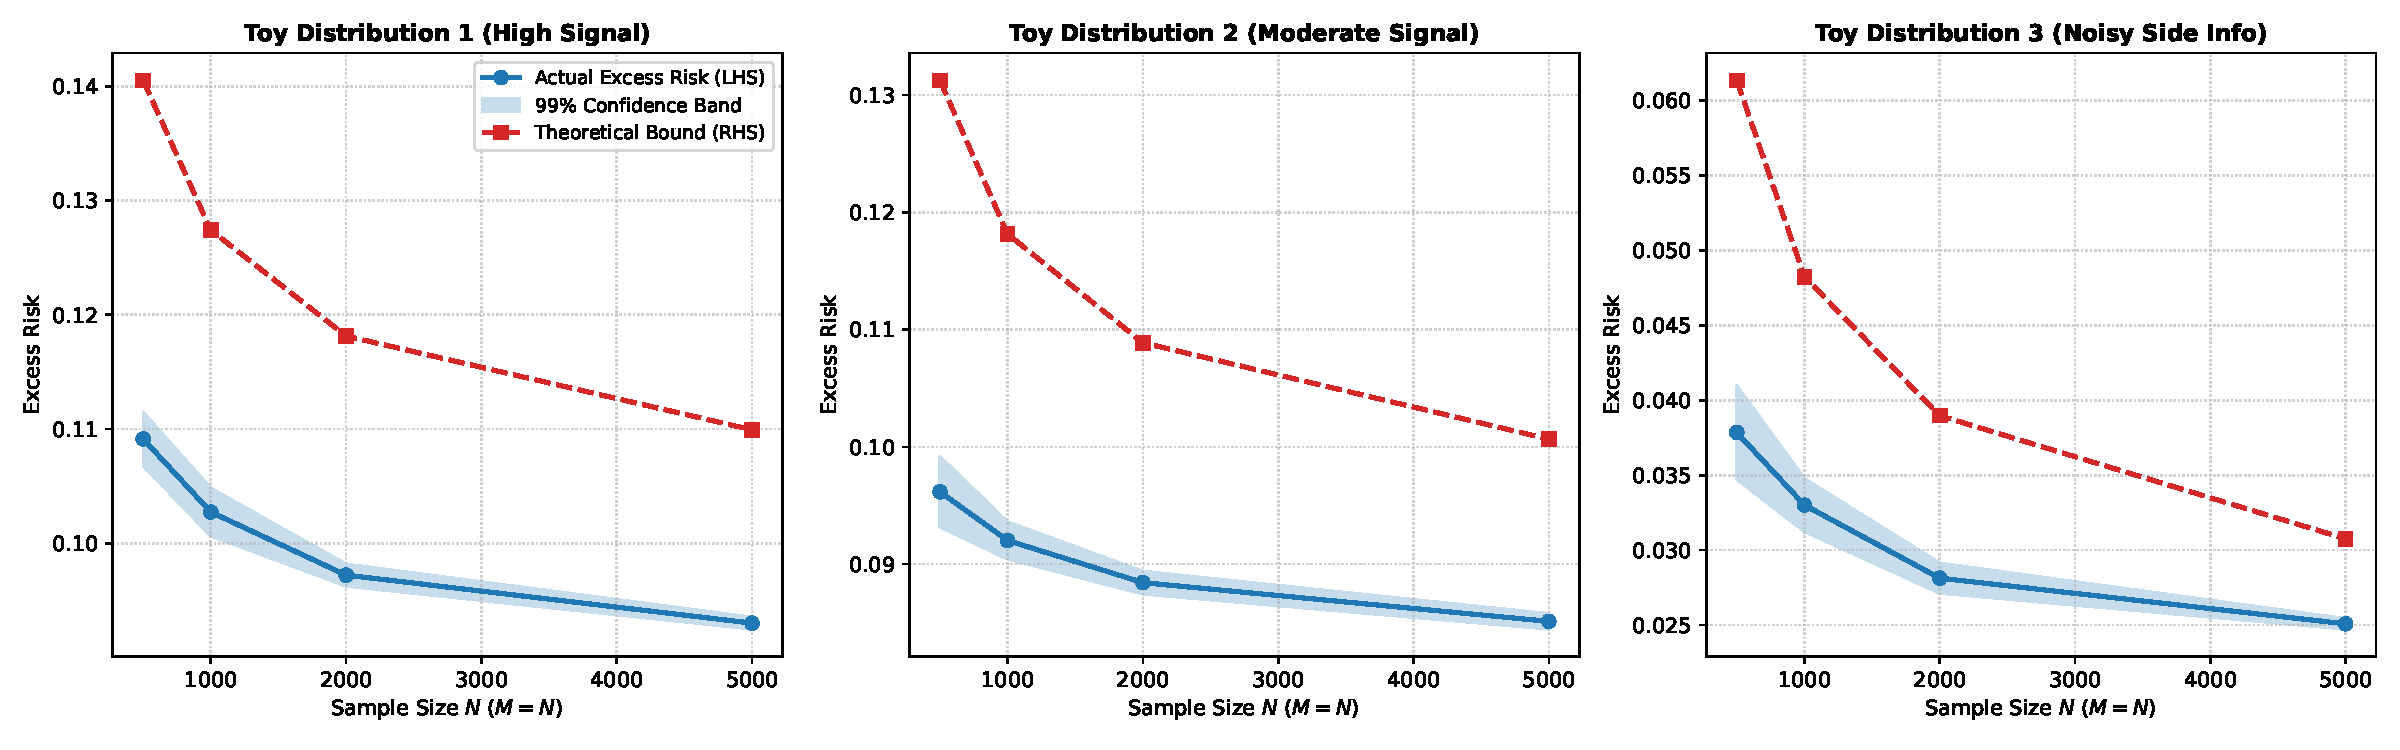
\includegraphics[width=\linewidth,height=3.4cm,keepaspectratio]{../Chapter_3_Side_Information/Figures/fig_excess_risk_toy.pdf}
\par{\scriptsize Excess risk across 3 signal regimes ($m=n$, 20 runs, 99\% CI). Actual excess risk closely tracks theoretical bound decay.}
\end{column}

\begin{column}{0.48\textwidth}
\centering
\textbf{Real-World Benchmark Datasets}
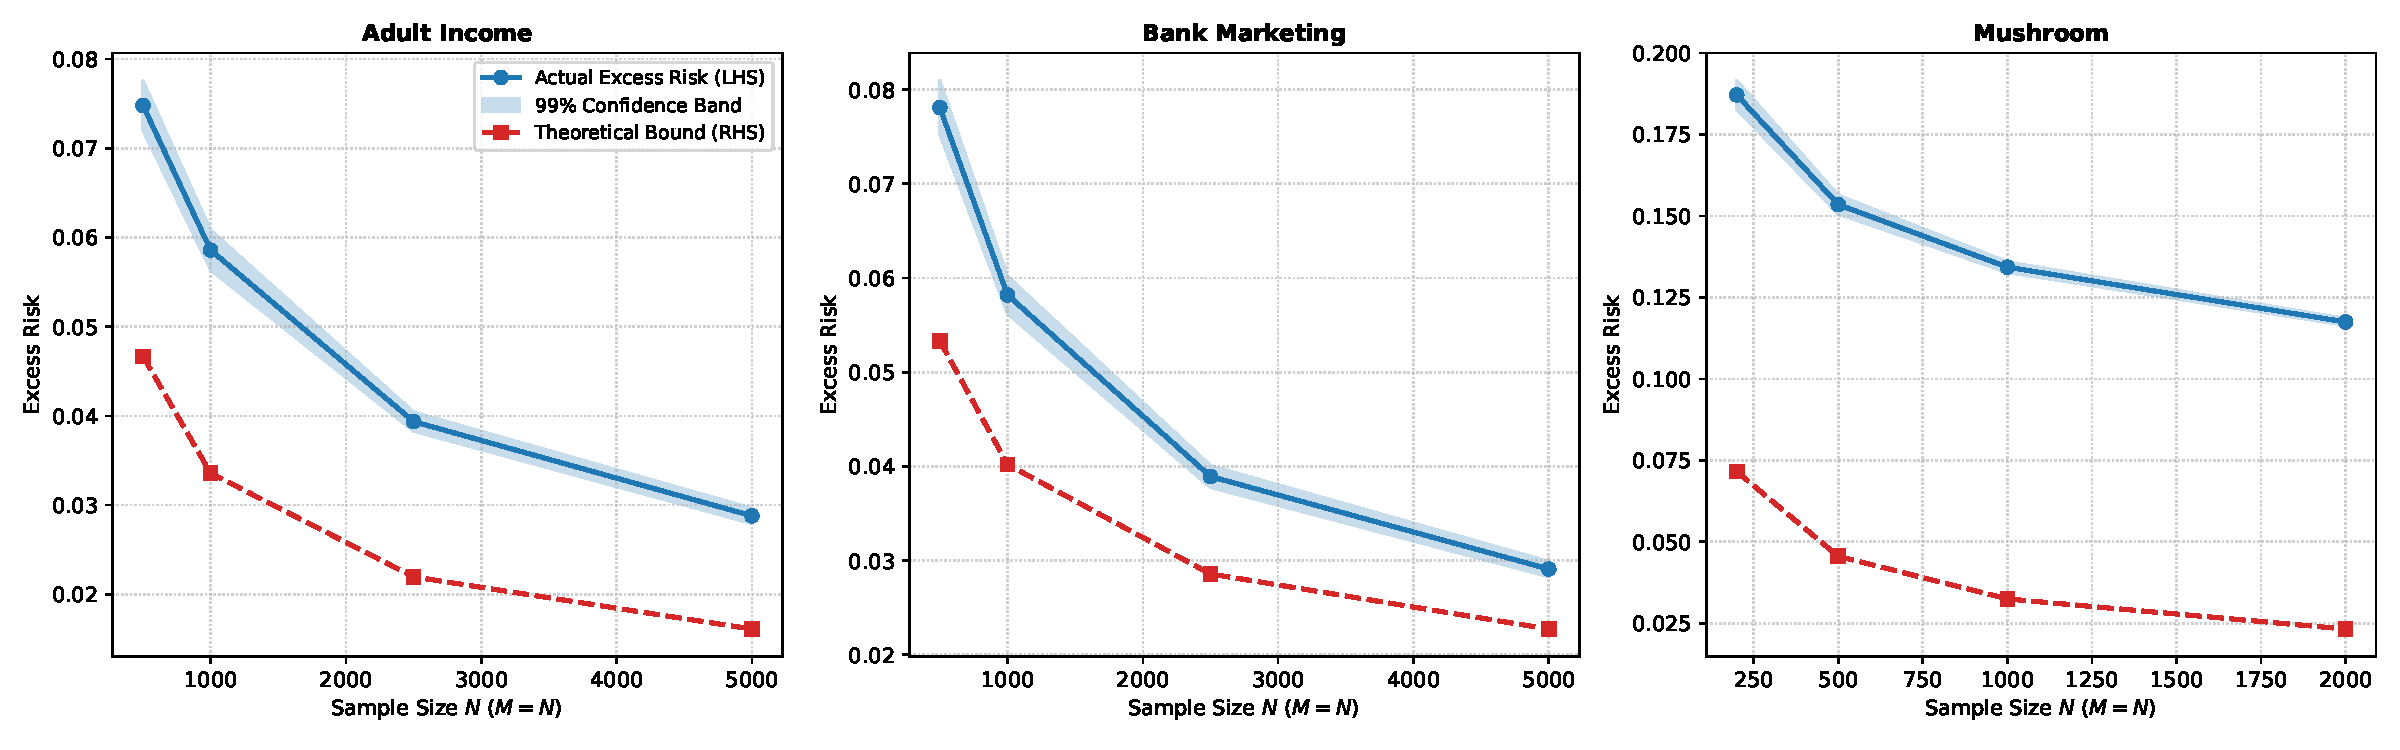
\includegraphics[width=\linewidth,height=3.4cm,keepaspectratio]{../Chapter_3_Side_Information/Figures/fig_excess_risk_real.pdf}
\par{\scriptsize OpenML datasets (Adult Income, Bank Marketing, Mushroom). Demonstrates consistent $1/\sqrt{n}$ decay trajectory across diverse real domains.}
\end{column}
\end{columns}
\end{frame}


% ══════════════════════════════════════════════════════════════════════════════
\section{Strategic Feature Revelation}
% ══════════════════════════════════════════════════════════════════════════════

% ── SLIDE: Ch4 Motivation & Setting ───────────────────────────────────────────
\begin{frame}{Strategic Feature Revelation: Motivation \& Setting}
\small
\textbf{Context: Strategic Information Disclosure}
\begin{itemize}\itemsep=0.5pt
  \footnotesize
  \item In many high-stakes interactions, agents strategically withhold or disclose verifiable evidence (e.g., job candidates presenting selective test scores, loan applicants disclosing assets, firms reporting ESG metrics).
  \item \textbf{Verifiability:} Features cannot be fabricated, but unfavorable features can be strategically concealed.
\end{itemize}

\vspace{0.1em}
\textbf{The Revelation Regimes}
\begin{itemize}\itemsep=0.5pt
  \footnotesize
  \item \textcolor{IITBNavy}{\textbf{Mandatory Disclosure (Vanilla Baseline):}} Receiver compels disclosure of all features; communication suffers from exogenous transmission loss / packet erasure with probability $q \in [0, 1)$.
  \item \textcolor{IITBGold!80!black}{\textbf{Voluntary Disclosure (Strategic Regime):}} Sender strategically decides whether to reveal $X$ or withhold it, balancing private utility against receiver prediction.
\end{itemize}

\vspace{0.1em}
\begin{alertblock}{The Central Question}
\centering
\emph{``Can a sender's strategic withholding of verifiable information ever be strictly advantageous to the receiver compared to mandatory disclosure?''}
\end{alertblock}
\end{frame}

% ── SLIDE: Ch4 Problem Formulation ───────────────────────────────────────────
\begin{frame}{Strategic Feature Revelation: Problem Formulation}
\small
\begin{itemize}\itemsep=1.5pt
  \item \textbf{Information Structure:} Nature draws state $(U, X, Y) \sim \env$ where $X \in \mathcal{X} \subset \R^d$ (verifiable features), $Y \in \R$ (true target), and $U \in \R$ (sender's private preference target).
  \item \textbf{Receiver Commitment:} Commits to linear rule $r_b(x) = b^\top x$ on revealed features, and default $r_b(\emptyset) = 0$ when withheld or erased.
  \item \textbf{Sender Action:} Chooses message $s \in \{X, \emptyset\}$ to minimize expected squared error $(r_b(m) - U)^2$.
  \item \textbf{Erasure Channel:} Revealed features are erased with probability $q \in [0,1)$: $\prob(m = \emptyset \mid s = X) = q$.
\end{itemize}

\vspace{0.3em}
\centering
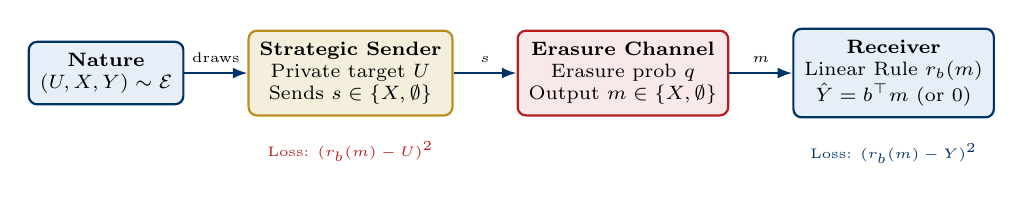
\begin{tikzpicture}[
  node distance=1.0cm and 0.8cm,
  box/.style={draw=IITBNavy, fill=IITBLight, rounded corners=3pt, thick, align=center, inner sep=4pt, font=\scriptsize},
  agent/.style={draw=IITBGold, fill=IITBGold!15, rounded corners=3pt, thick, align=center, inner sep=4pt, font=\scriptsize},
  channel/.style={draw=DarkRed, fill=DarkRed!10, rounded corners=3pt, thick, align=center, inner sep=4pt, font=\scriptsize},
  arrow/.style={-{Latex[scale=0.8]}, thick, draw=IITBNavy}
]
  \node[box] (nature) {\textbf{Nature}\\$(U, X, Y) \sim \env$};
  \node[agent, right=0.8cm of nature] (sender) {\textbf{Strategic Sender}\\Private target $U$\\Sends $s \in \{X, \emptyset\}$};
  \node[channel, right=0.8cm of sender] (channel) {\textbf{Erasure Channel}\\Erasure prob $q$\\Output $m \in \{X, \emptyset\}$};
  \node[box, right=0.8cm of channel] (receiver) {\textbf{Receiver}\\Linear Rule $r_b(m)$\\$\hat{Y} = b^\top m$ (or $0$)};

  \draw[arrow] (nature) -- node[above, font=\tiny] {draws} (sender);
  \draw[arrow] (sender) -- node[above, font=\tiny] {$s$} (channel);
  \draw[arrow] (channel) -- node[above, font=\tiny] {$m$} (receiver);

  \node[below=0.2cm of sender, font=\tiny, align=center, text=DarkRed] {Loss: $(r_b(m) - U)^2$};
  \node[below=0.2cm of receiver, font=\tiny, align=center, text=IITBNavy] {Loss: $(r_b(m) - Y)^2$};
\end{tikzpicture}
\end{frame}

% ── SLIDE: Ch4 Best Response & Strategic Advantage ───────────────────────────
\begin{frame}{Decision Problem: Sender Response \& Strategic Advantage}
\small
\textbf{Sender Best Response ($q < 1$):}
\begin{itemize}\itemsep=0.5pt
  \footnotesize
  \item Sender reveals $s = X$ if $\E[(r_b(m) - U)^2 \mid s = X] < \E[(r_b(m) - U)^2 \mid s = \emptyset]$.
  \item $(1-q)(b^\top X - U)^2 + q U^2 < U^2 \iff (2U - b^\top X) b^\top X > 0$.
  \item Defining $F_b(u, x) \coloneqq (2u - b^\top x) b^\top x$, sender reveals iff $\mathbf{F_b(U, X) > 0}$.
\end{itemize}

\vspace{0.1em}
\textbf{Receiver Risks \& Strategic Advantage:}
\begin{itemize}\itemsep=0.5pt
  \footnotesize
  \item \textbf{Vanilla Risk:} $R_V(b) = q\E[Y^2] + (1-q)\E[(Y - b^\top X)^2]$; optimal $b_V = \operatorname{Var}(X)^{-1} \operatorname{Cov}(X,Y)$.
  \item \textbf{Strategic Risk:} $R_S(b) = \E[Y^2] - (1-q)\E[G_b(X,Y) \I{F_b(U,X) > 0}]$, with $G_b(x, y) \coloneqq (2y - b^\top x) b^\top x$.
\end{itemize}

\vspace{0.1em}
\begin{block}{Strategic Advantage \& Channel Invariance}
\footnotesize
\[
  \Delta(\env) \coloneqq \inf_b R_V(b) - \inf_b R_S(b) = (1-q) \Delta(0).
\]
\textbf{Key Invariance:} The erasure channel scales the magnitude of $\Delta$ by $(1-q)$, but \textbf{strictly preserves its sign} for all $q < 1$!
\end{block}
\end{frame}

% ── SLIDE: Ch4 Conditions for Strategic Advantage ─────────────────────────────
\begin{frame}{Conditions for Positive Strategic Advantage ($\Delta > 0$)}
\small
\begin{columns}[T,onlytextwidth]
\begin{column}{0.51\textwidth}
\footnotesize
Assume centered variables and finite 2nd moments. Define:
\[
  A(b) \coloneqq \E|G_b| - \operatorname{Var}(b_V^\top X) - \operatorname{Var}((b - b_V)^\top X).
\]

\vspace{0.1em}
\begin{block}{Theorems 4.3 \& 4.4 (Advantage Conditions)}
\begin{itemize}\itemsep=2pt
  \item \textbf{Necessary:} $\Delta(\env) > 0 \implies \exists b : A(b) > 0$.
  \item \textbf{Sufficient (Preference Alignment):}
  \[
    \exists b : \|U - Y\|_2 < \frac{A(b)}{4\sqrt{\operatorname{Var}(b^\top X)}} \implies \mathbf{\Delta(\env) > 0}.
  \]
\end{itemize}
\end{block}
\par{\scriptsize \textbf{Interpretation:} When preferences are aligned, withholding acts as an informative non-linear filter, improving prediction!}
\end{column}

\begin{column}{0.47\textwidth}
\centering
\textbf{Parameter Sweep: Advantage Region}
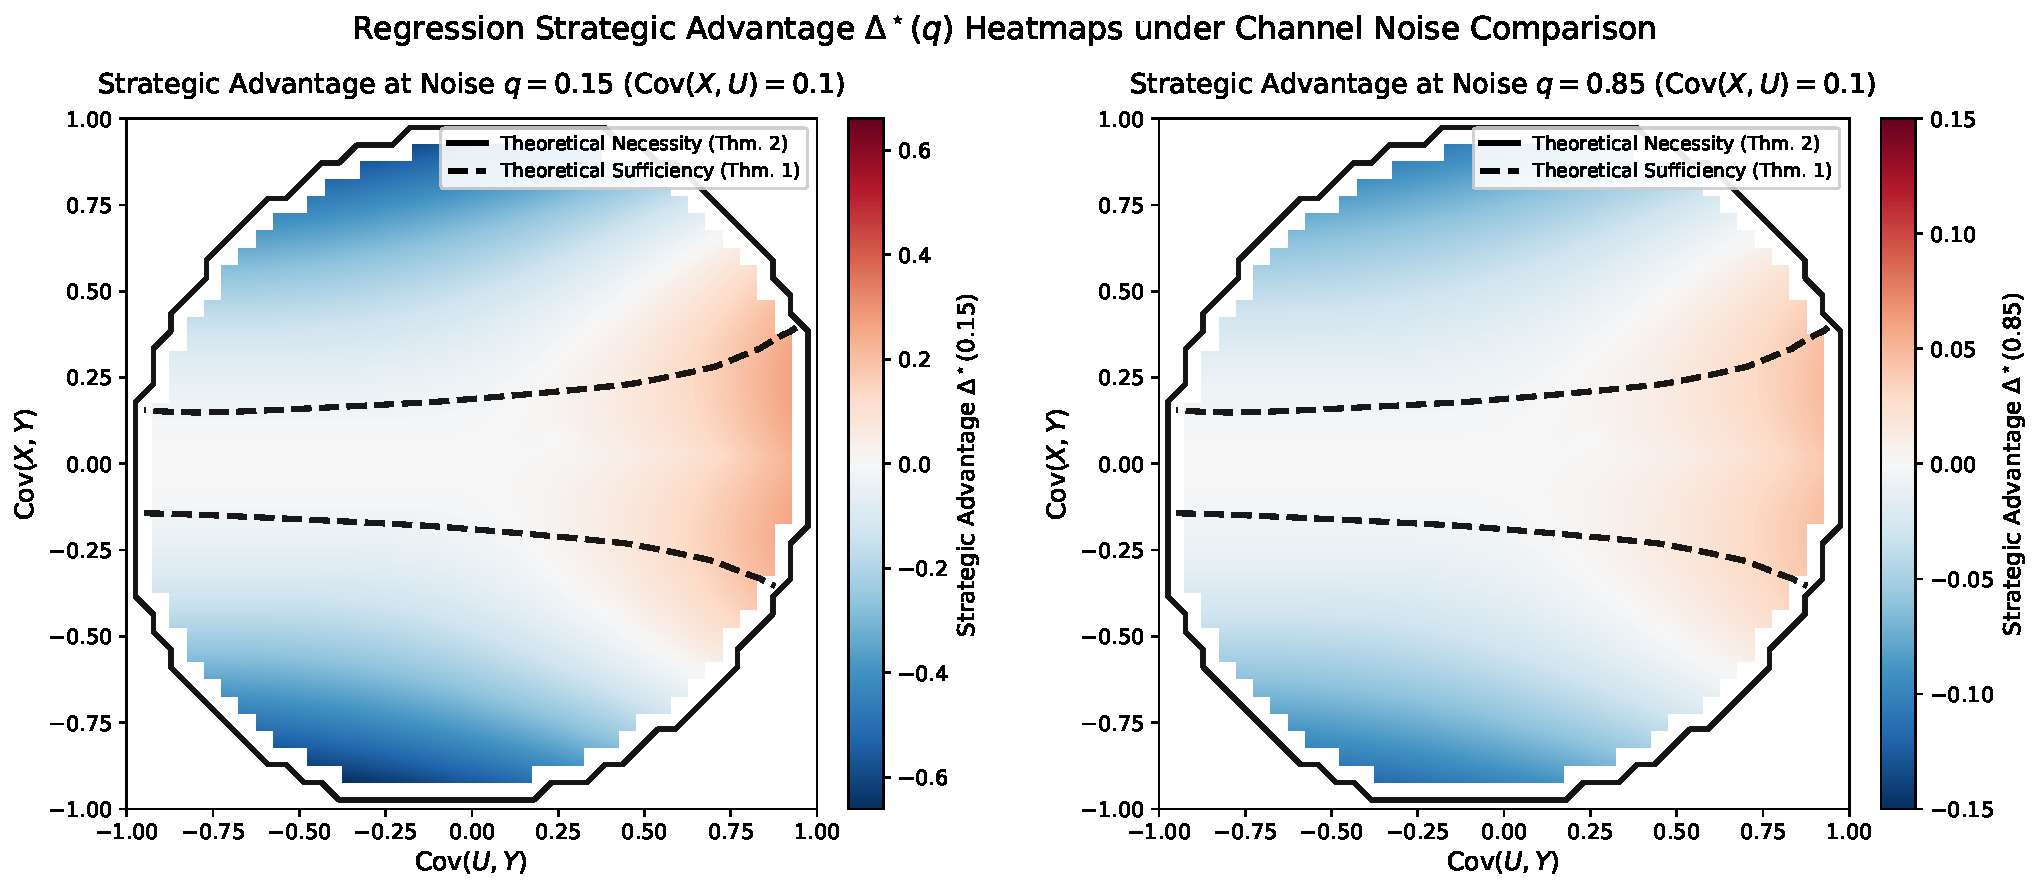
\includegraphics[width=\linewidth,height=3.3cm,keepaspectratio]{../Chapter_4_Strategic_Revelation/figures/regression_decision_sweep.pdf}
\par{\scriptsize Parameter sweep across alignment $\|U-Y\|_2$ and variance, identifying the strictly positive strategic advantage regime ($\Delta(\env) > 0$).}
\end{column}
\end{columns}
\end{frame}

% ── SLIDE: Ch4 Offline Learning ───────────────────────────────────────────────
\begin{frame}{Offline Learning: Strategy-Aware Regression ERM}
\small
\begin{columns}[T,onlytextwidth]
\begin{column}{0.54\textwidth}
\scriptsize
\textbf{Unknown Law, Finite Training Sample:}
$D_n = \{(U_i, X_i, Y_i)\}_{i=1}^n \stackrel{\text{i.i.d.}}{\sim} \env$ with $\|X\|_2, |U|, |Y| \le 1$.

\textbf{SAR-ERM Estimators:}
\setlength{\abovedisplayskip}{2pt}
\setlength{\belowdisplayskip}{2pt}
\begin{align*}
  \widehat{R}_V(b) &= \tfrac{1}{n} \sum_{i=1}^n \bigl[ q Y_i^2 + (1-q)(Y_i - b^\top X_i)^2 \bigr], \\
  \widehat{R}_S(b) &= \tfrac{1}{n} \sum_{i=1}^n \bigl[ Y_i^2 - (1-q) G_b(X_i, Y_i) \I{F_b > 0} \bigr].
\end{align*}
$\widehat{\Delta} = \inf_{\|b\|_2 \le 1} \widehat{R}_V(b) - \inf_{\|b\|_2 \le 1} \widehat{R}_S(b)$.

\begin{block}{Theorem 4.6 (Uniform Generalization Bound)}
\scriptsize
With probability at least $1 - \delta$:
\setlength{\abovedisplayskip}{2pt}
\setlength{\belowdisplayskip}{2pt}
\[
  |\Delta(\env) - \widehat{\Delta}| \le \widetilde{\mathcal{O}}\left(\frac{d^3}{\sqrt{n}} + \frac{d^2 \sqrt{\log(1/\delta)}}{\sqrt{n}}\right).
\]
\end{block}
\end{column}

\begin{column}{0.44\textwidth}
\centering
\textbf{Empirical Generalization Gaps}
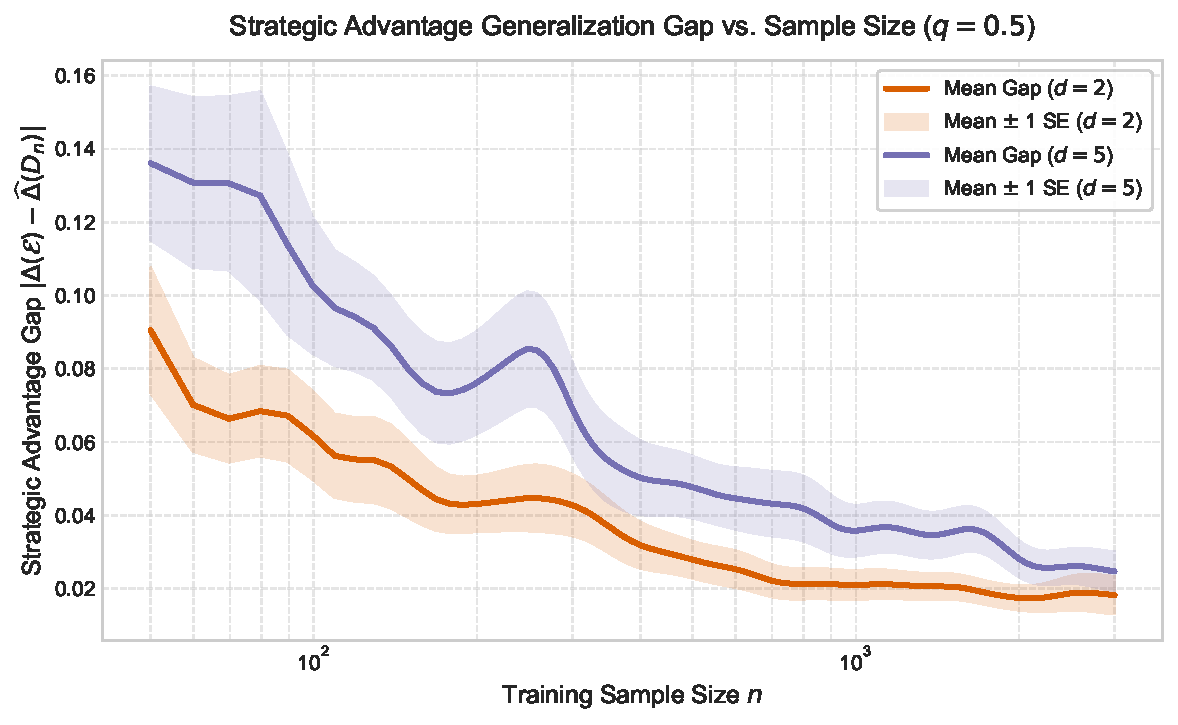
\includegraphics[width=\linewidth,height=2.5cm,keepaspectratio]{../Chapter_4_Strategic_Revelation/figures/regression_learning_gaps.pdf}
\par{\scriptsize Error gaps $|\Delta - \widehat{\Delta}|$ across sample sizes $n$, confirming parametric $\mathcal{O}(1/\sqrt{n})$ rate.}
\end{column}
\end{columns}
\end{frame}

% ── SLIDE: Ch4 Online Learning ────────────────────────────────────────────────
\begin{frame}{Online Learning: Joint Regime and Slope Selection}
\small
\textbf{Sequential Interaction Protocol:} At each round $t = 1, \dots, T$:
\begin{enumerate}\itemsep=2pt
  \item Receiver commits to joint action $a_t = (m_t, b_t) \in \{V, S\} \times \mathcal{B}_d(1)$ (regime and slope).
  \item Nature draws $(U_t, X_t, Y_t) \sim \env$; sender reveals if $m_t = V$ or ($m_t = S$ and $F_{b_t} > 0$).
  \item Receiver observes \textbf{bandit loss feedback}: single realized squared error $Z_t = \ell(r_{a_t}, Y_t) + \eta_t$.
\end{enumerate}

\vspace{0.4em}
\textbf{Composite Kernel Gaussian Process Thompson Sampling (GP-TS):}
\begin{itemize}\itemsep=2pt
  \item Model expected loss $f(m,b) = \E[Z \mid a=(m,b)]$ with composite Mat\'ern-$5/2$ covariance:
  \[
    k((m,b), (m',b')) = \mathbbm{1}_{\{m=m'\}} \cdot k_{5/2}(b, b').
  \]
  Decouples vanilla and strategic regimes while preserving shared smoothness properties.
  \item \textbf{Algorithm:} Maintain posterior $\mathcal{GP}(\mu_{t-1}, k_{t-1})$; draw inflated sample $\widetilde{f}_t \sim \mathcal{GP}(\mu_{t-1}, v_t^2 k_{t-1})$; select $a_t = \arg\min_{a \in \mathcal{A}_t} \widetilde{f}_t(a)$ over discretization net; observe $Z_t$ and update posterior.
\end{itemize}
\end{frame}

% ── SLIDE: Ch4 Online Regret & Simulation ─────────────────────────────────────
\begin{frame}{Online Regret Guarantee \& Empirical Validation}
\small
\begin{columns}[T,onlytextwidth]
\begin{column}{0.50\textwidth}
\begin{block}{Theorem 4.10 (Sublinear Cumulative Regret)}
\scriptsize
Assume regime risks lie in Mat\'ern-$5/2$ RKHS with $\|f\|_{\mathcal{H}} \le B$, and noise is conditionally sub-Gaussian. Then GP-TS achieves:
\setlength{\abovedisplayskip}{2pt}
\setlength{\belowdisplayskip}{2pt}
\[
  \operatorname{Reg}_T = \sum_{t=1}^T \bigl[f(a_t) - \inf_a f(a)\bigr] = \widetilde{\mathcal{O}}\left( T^{\frac{5+3d}{10+2d}} \right).
\]
\end{block}

\textbf{Sublinear Exponent Across Dimension:}
\begin{center}
\scriptsize
\begin{tabular}{ccccc}
\toprule
$d=1$ & $d=2$ & $d=3$ & $d=4$ & $d \ge 5$ \\
\midrule
$T^{0.67}$ & $T^{0.79}$ & $T^{0.88}$ & $T^{0.94}$ & Linear \\
\bottomrule
\end{tabular}
\end{center}
\par{\scriptsize \textbf{Takeaway:} Sublinear regret $\operatorname{Reg}_T/T \to 0$ holds for all $d \le 4$, establishing online learnability.}
\end{column}

\begin{column}{0.48\textwidth}
\centering
\textbf{Cumulative Regret Trajectories}
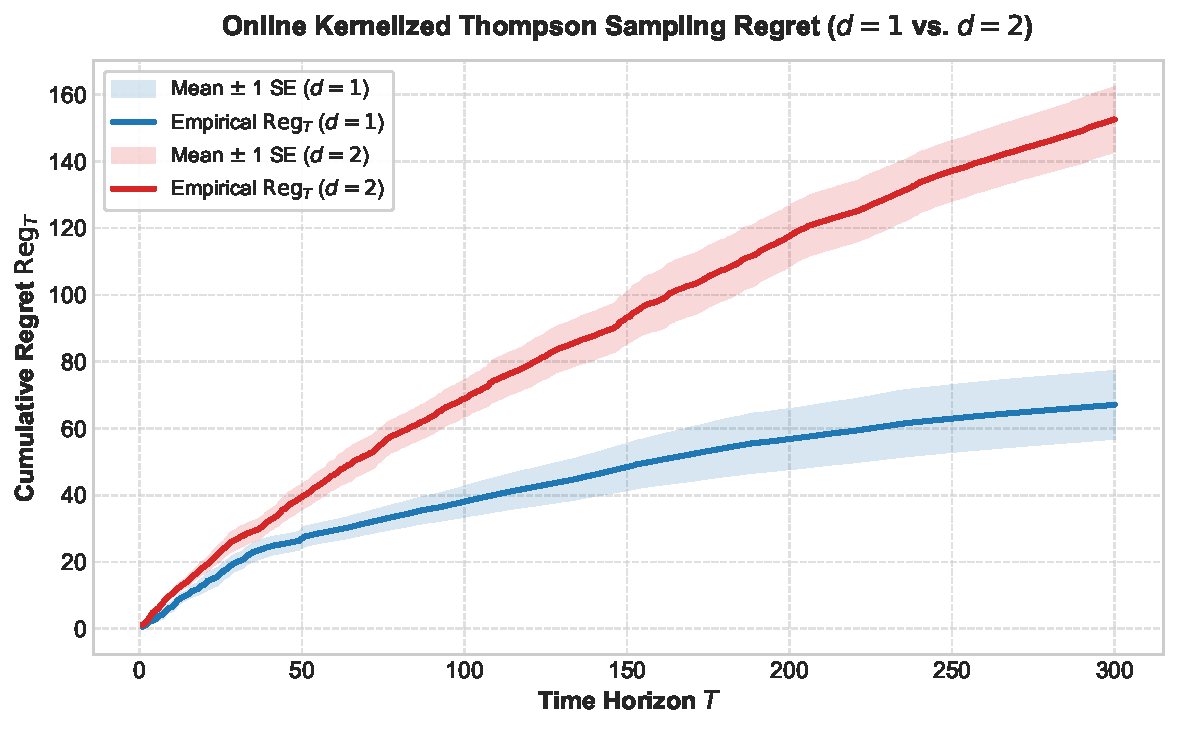
\includegraphics[width=\linewidth,height=2.6cm,keepaspectratio]{../Chapter_4_Strategic_Revelation/figures/online_learning_regret.pdf}
\par{\scriptsize Cumulative regret curves for $d=1, 2$ across rounds $T$, exhibiting sublinear empirical scaling in accordance with Theorem 4.10.}
\end{column}
\end{columns}
\end{frame}


% ══════════════════════════════════════════════════════════════════════════════
\section{Strategic IPO Regulation}
% ══════════════════════════════════════════════════════════════════════════════

% ── SLIDE: Ch5 Motivation & Setting ───────────────────────────────────────────
\begin{frame}{Strategic IPO Regulation: Motivation \& Setting}
\small
\textbf{Economic Context: Initial Public Offerings (IPOs)}
\begin{itemize}\itemsep=1.5pt
  \item Private firms raise public equity capital by selling shares to retail and institutional investors.
  \item \textbf{Information Asymmetry:} Issuing firms possess private knowledge of true productivity $Y(X)$, but present self-selected marketing disclosures, metrics, and projections $z$.
\end{itemize}

\vspace{0.2em}
\textbf{Regulatory Dilemma: The Tolerance Parameter $\varepsilon$}
\begin{itemize}\itemsep=1.5pt
  \item Regulators enforce disclosure standards restricting presentation deviation: $\|z - X\|_2 \le \varepsilon$.
  \item \textcolor{IITBNavy}{\textbf{Zero Tolerance ($\varepsilon \to 0$):}} Eliminates misrepresentation, but creates severe compliance frictions and suppresses capital formation.
  \item \textcolor{IITBGold!80!black}{\textbf{Lax Tolerance ($\varepsilon \to \infty$):}} Maximizes trading liquidity, but induces severe lemon-market adverse selection and misallocation.
\end{itemize}

\vspace{0.2em}
\begin{alertblock}{The Central Policy Question}
\centering
\emph{``How should a regulator set tolerance $\varepsilon$ to balance capital formation against adverse selection when firms strategically window-dress their presentations?''}
\end{alertblock}
\end{frame}

% ── SLIDE: Ch5 Problem Formulation ───────────────────────────────────────────
\begin{frame}{Strategic IPO Regulation: Problem Formulation}
\small
\textbf{Game Primitives:}
\begin{itemize}\itemsep=0.5pt
  \footnotesize
  \item \textbf{Firm:} Fundamentals $X \in \mathcal{X} \subset \R^d$, true productivity $Y(X) \in \R_+$.
  \item \textbf{Regulator:} Announces tolerance $\varepsilon \ge 0$ prior to firm realization.
  \item \textbf{Firm Action:} Chooses presentation $z \in \mathcal{X}$ with $\|z - X\|_2 \le \varepsilon$ and share price $P \ge 0$.
\end{itemize}

\vspace{0.1em}
\textbf{Market Demand \& Investor Heterogeneity:}
\begin{itemize}\itemsep=0.5pt
  \footnotesize
  \item $k$ heterogeneous investor subpopulations $j \in \{1, \dots, k\}$ with sizes $N_j$ and valuations $V_j(z)$; total pool $\mathcal{N} = \sum_{j=1}^k N_j$.
  \item Traded volume under issuance cap $\eta \in (0,1]$:
  $Q(z, P) = \min\big\{\eta\mathcal{N},\; \sum_{j=1}^k N_j \mathbbm{1}_{\{V_j(z) \ge P\}}\big\}$.
\end{itemize}

\vspace{0.1em}
\textbf{Objectives:}
\begin{itemize}\itemsep=0.5pt
  \footnotesize
  \item \textbf{Firm:} Maximizes total capital proceeds $\Pi(z, P) = P \cdot Q(z, P)$.
  \item \textbf{Regulator:} Maximizes expected social welfare $\mathcal{W}(\varepsilon) = \E\left[ \frac{Q^*(X, \varepsilon) \cdot Y(X)}{\mathcal{N}} \right]$.
\end{itemize}
\end{frame}

% ── SLIDE: Ch5 Firm Strategy & Saturation ─────────────────────────────────────
\begin{frame}{Decision Problem: Convex Decomposition \& Saturation}
\small
\begin{block}{Theorem 5.2 (Convex Decomposition of Firm Optimal Response)}
\footnotesize
For fixed presentation $z$, optimal price satisfies $P \in \{0\} \cup \{V_j(z) : V_j(z) \ge 0\}$.
The firm's joint optimization reduces to solving at most $2^k - 1$ convex programs:
\[
  \max_{z \in \mathcal{X}, P \ge 0} P \cdot \E\left[\min\!\left\{\eta\mathcal{N}, \sum_{j \in S} N_j\right\} \;\middle|\; X=x\right] \quad \text{s.t.} \quad \|z - x\|_2 \le \varepsilon, \; P \le V_j(z) \; \forall j \in S.
\]
For concave valuations $V_j$, each subproblem is a convex program. The firm chooses the revenue-maximizing subset $S^\star \subseteq \{1, \dots, k\}$.
\end{block}

\vspace{0.15em}
\begin{block}{Proposition 5.3 (Saturation beyond $\varepsilon_{\max}$)}
\footnotesize
For $\varepsilon \ge \operatorname{diam}(\mathcal{X})$, the ball $\mathcal{B}(x, \varepsilon)$ covers all of $\mathcal{X}$. Welfare $\mathcal{W}(\varepsilon)$ saturates to a constant $\mathcal{W}(\varepsilon_{\max})$.
\end{block}

\vspace{0.1em}
\textbf{Interior Optimum Criterion:}\par
If $\mathcal{W}'(0) > 0$ and $\mathcal{W}'(\varepsilon_{\max}) < 0$, the optimal policy $\varepsilon^\star$ is strictly interior:
$\varepsilon^\star \in (0, \varepsilon_{\max})$ satisfying $\mathcal{W}'(\varepsilon^\star) = 0$.
\end{frame}

% ── SLIDE: Ch5 Affine Example & Decision Sim ──────────────────────────────────
\begin{frame}{Decision Problem: Affine Valuations \& Targeting}
\small
\textbf{Bimodal Market ($k=2$):} Groups $\alpha, \beta$ with equal mass $N_\alpha = N_\beta = \mathcal{N}/2$, full supply $\eta = 1$.
Valuations: $V_\alpha(z) = w_\alpha^\top z + b_\alpha$ and $V_\beta(z) = w_\beta^\top z + b_\beta$.
\begin{itemize}\itemsep=1pt
  \item \textbf{Target $\alpha$ or $\beta$ alone:} $P_j^*(x, \varepsilon) = V_j(x) + \varepsilon \|w_j\|_2$, Traded Volume $Q = \mathcal{N}/2$.
  \item \textbf{Target both (Pooling):} $P_{\alpha\beta}^*(x, \varepsilon) = \max_{\|\Delta\|_2 \le \varepsilon} \min\{V_\alpha(x+\Delta), V_\beta(x+\Delta)\}$, Volume $Q = \mathcal{N}$.
\end{itemize}

\vspace{0.2em}
\begin{columns}[T,onlytextwidth]
\begin{column}{0.48\textwidth}
\centering
\textbf{Analytical Welfare Curve}
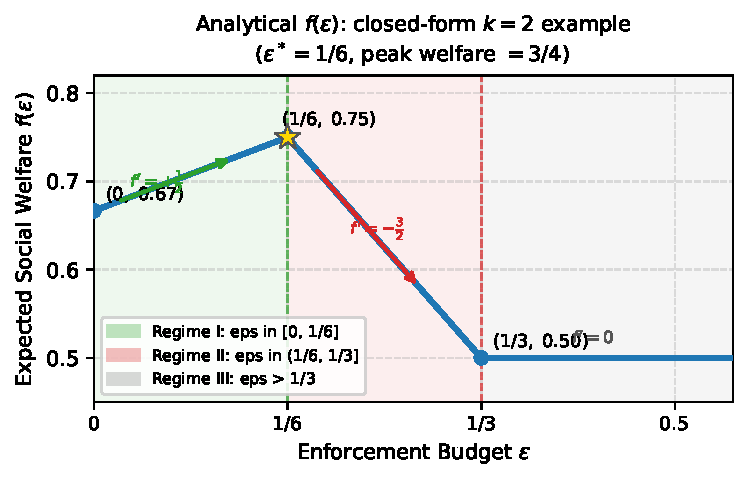
\includegraphics[width=\linewidth,height=3.2cm,keepaspectratio]{../Chapter_5_IPO/figures/feps_analytical.pdf}
\par{\scriptsize Analytical welfare $\mathcal{W}(\varepsilon)$ exhibiting non-monotonicity and interior optimal tolerance $\varepsilon^\star$.}
\end{column}

\begin{column}{0.48\textwidth}
\centering
\textbf{Market Simulation Results}
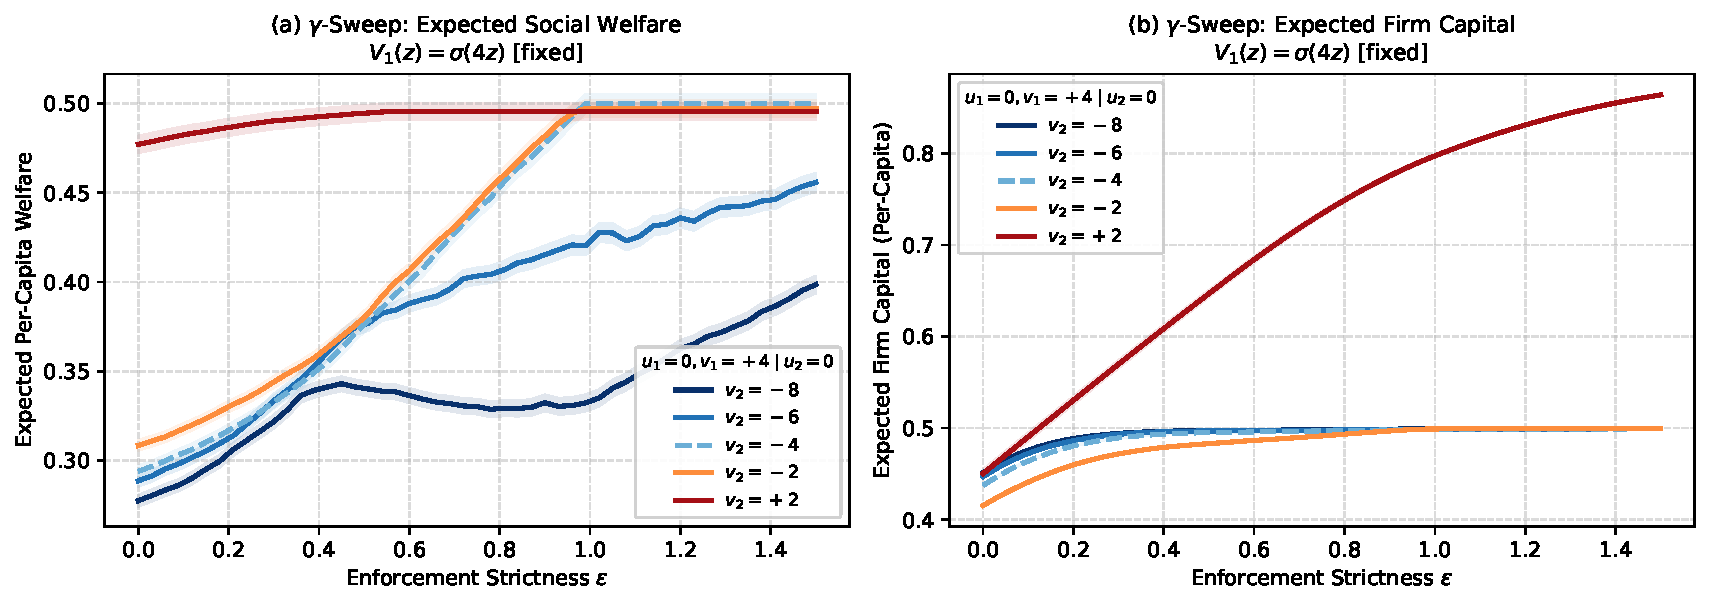
\includegraphics[width=\linewidth,height=3.2cm,keepaspectratio]{../Chapter_5_IPO/figures/decision_sim_results.pdf}
\par{\scriptsize Welfare $\mathcal{W}(\varepsilon)$ and traded volume $Q(\varepsilon)$ vs tolerance $\varepsilon$, showing initial gains before degradation.}
\end{column}
\end{columns}
\end{frame}

% ── SLIDE: Ch5 Online Learning ────────────────────────────────────────────────
\begin{frame}{Online IPO Regulation: GP-TS \& Regret Guarantee}
\small
\begin{columns}[T,onlytextwidth]
\begin{column}{0.52\textwidth}
\scriptsize
\textbf{Unknown Market Distribution:}
Regulator selects tolerance $\varepsilon_t \in [0, \varepsilon_{\max}]$ over rounds $t = 1, \dots, T$; observes noisy welfare $W_t = \mathcal{W}(\varepsilon_t) + \xi_t$.

\vspace{0.1em}
\textbf{Algorithm: Mat\'ern-$5/2$ GP-TS}
\begin{itemize}\itemsep=0.5pt
  \item Maintain GP posterior over $[0, \varepsilon_{\max}]$.
  \item Draw inflated sample and maximize over net.
  \item Update posterior with realized market welfare $W_t$.
\end{itemize}

\vspace{0.05em}
\begin{block}{Theorem 5.5 (Online Regret Bound)}
\scriptsize
Assuming welfare $\mathcal{W} \in \mathcal{H}_k(B)$ and sub-Gaussian noise:
\[
  R_T = \sum_{t=1}^T \bigl[\mathcal{W}(\varepsilon^\star) - \mathcal{W}(\varepsilon_t)\bigr] = \mathbf{\widetilde{\mathcal{O}}\left(T^{2/3}\right)}.
\]
\end{block}
\par{\scriptsize \textbf{Takeaway:} Sublinear regret guarantees convergence to optimal regulatory policy despite window-dressing.}
\end{column}

\begin{column}{0.46\textwidth}
\centering
\textbf{Online Learning Regret}
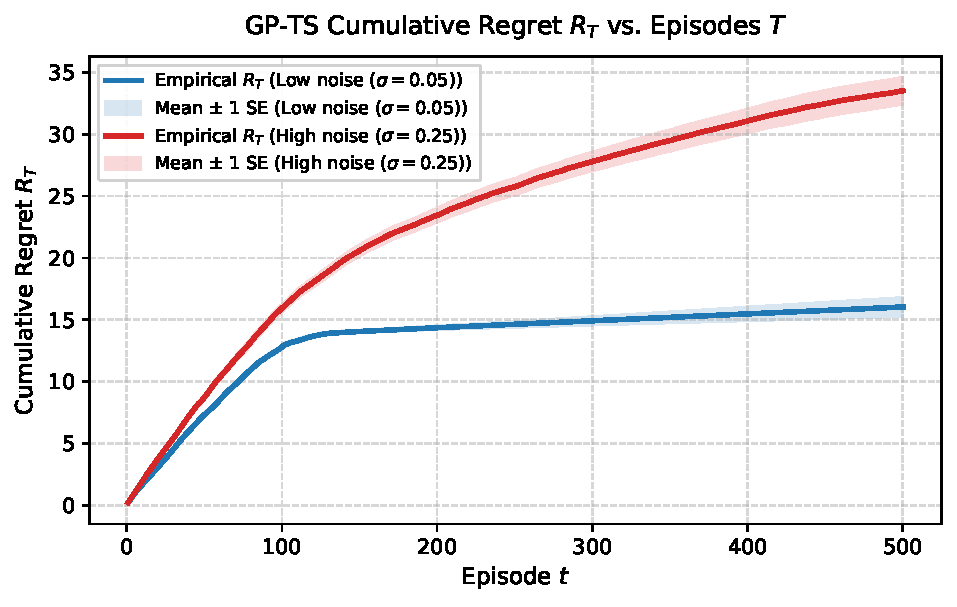
\includegraphics[width=\linewidth,height=2.8cm,keepaspectratio]{../Chapter_5_IPO/figures/learning_results.pdf}
\par{\scriptsize Cumulative regret of GP Thompson Sampling compared to naive fixed tolerances, showing sublinear convergence.}
\end{column}
\end{columns}
\end{frame}


% ══════════════════════════════════════════════════════════════════════════════
\section{Conclusion}
% ══════════════════════════════════════════════════════════════════════════════

% ── SLIDE: Cross-Chapter Synthesis ───────────────────────────────────────────
\begin{frame}{Cross-Chapter Results}
\small
\begin{description}
\item[Chapter 2] Penalty labels and randomization alter strategic response.
Learning depends on the complexity of the induced classification rules.
\item[Chapter 3] Imputation and regularization balance the value of side information
against missing joint observations. Some information remains unidentified.
\item[Chapter 4] Explicit conditions identify when voluntary disclosure can improve
regression. Offline estimation and online regret require their stated assumptions.
\item[Chapter 5] The firm problem reduces to buyer-subset programs.
Regulatory learning has a conditional Mat\'ern GP-TS regret guarantee.
\end{description}
\end{frame}

% ── SLIDE: Key Takeaway ─────────────────────────────────────────────────────
\begin{frame}{Incentives and Observations Shape Learning}
\small
\textbf{Strategic response changes the decision problem.}
\begin{itemize}
\item A penalty or a randomized rule changes the incentive to manipulate.
\item A disclosure choice carries information about a sender's preferences.
\item A firm's response connects regulatory tolerance to pricing and participation.
\end{itemize}
\par\vspace{.8em}
\textbf{The observation structure changes what can be learned.}
\begin{itemize}
\item Partitioned samples can leave dependencies unidentified.
\item Bandit feedback reveals only the outcome of the chosen action.
\item Guarantees depend on the function class, the feedback model and the comparator.
\end{itemize}
\end{frame}

% ── SLIDE: Publications ──────────────────────────────────────────────────────
\begin{frame}{Publications Arising from this Dissertation}
\footnotesize
\textbf{Journal Articles:}
\begin{enumerate}
  \item \textbf{M.~K.~Singh} and A.~A.~Kulkarni. ``Strategic Classification for Non-uniform Preferences using Penalty Labels and Randomisation,'' \emph{Autonomous Agents and Multi-Agent Systems (JAAMAS)}, 2025.
  \item \textbf{M.~K.~Singh}, S.~S.~Kowshik, and A.~A.~Kulkarni. ``Learning with Side Information from Partitioned Data,'' \emph{Information and Inference: A Journal of the IMA} (Oxford University Press), (\emph{Submitted}).
  \item \textbf{M.~K.~Singh}, A.~A.~Kulkarni, and K.~Mahajan. ``Learning under Strategic Feature Revelation,'' (\emph{Submitted to Journal}).
  \item \textbf{M.~K.~Singh} and A.~A.~Kulkarni. ``Strategic IPO Regulation under Complete and Incomplete Information,'' (\emph{Submitted to Journal}).
\end{enumerate}

\par\vspace{0.2em}
\textbf{Conference Proceedings:}
\begin{enumerate}
  \item \textbf{M.~K.~Singh}, A.~A.~Kulkarni, and K.~Mahajan. ``Learning under Strategic Feature Revelation,'' \emph{IEEE Conference on Decision and Control (CDC)}, 2026 (\emph{Accepted}).
  \item \textbf{M.~K.~Singh} and A.~A.~Kulkarni. ``Optimal Stochastic Decision Rule for Strategic Classification,'' \emph{National Conference on Communications (NCC)}, 2024.
  \item \textbf{M.~K.~Singh} and A.~A.~Kulkarni. ``Strategic Multiclass Classification with Non-uniform Preferences and its Relation to Incentive Compatibility,'' \emph{Indian Control Conference (ICC)}, 2022 (\emph{Best Student Paper Award}).
\end{enumerate}
\end{frame}

% ── SLIDE: Future Directions ─────────────────────────────────────────────────
\begin{frame}{Future Research Directions}
\small
\begin{itemize}
  \item \textbf{Richer Strategic Models:}
  \begin{itemize}
    \item Multi-round repeated interactions and dynamic feature gaming.
    \item Multi-agent competition with heterogeneous decision makers.
    \item Non-linear hypothesis spaces with partial feature revelation.
  \end{itemize}

  \vspace{0.2em}
  \item \textbf{Bridging Strategic Decisions \& Partitioned Observations:}
  \begin{itemize}
    \item Strategic agents operating under partitioned or incomplete information structures.
    \item Incentive-compatible imputation mechanism design.
  \end{itemize}

  \vspace{0.2em}
  \item \textbf{Policy \& Applied Systems:}
  \begin{itemize}
    \item Regulatory design in financial credit scoring, college admissions, and hiring algorithms.
    \item Structurally heterogeneous and federated multi-institution learning.
  \end{itemize}
\end{itemize}
\end{frame}

% ── SLIDE: References ────────────────────────────────────────────────────────
\begin{frame}{Major References}
\scriptsize
\begin{columns}[T,onlytextwidth]
\begin{column}{0.48\textwidth}
\textbf{Strategic Classification \& Learning}
\begin{itemize}\itemsep=3pt
  \item M.~Br\"uckner and T.~Scheffer. ``Stackelberg games for active learning.'' \emph{AISTATS}, 2011.
  \item M.~Hardt, N.~Megiddo, C.~Papadimitriou, and M.~Wootters. ``Strategic classification.'' \emph{ITCS}, 2016.
  \item R.~Sundaram, A.~Vullikanti, H.~Xu, and F.~Yao. ``PAC-learning for strategic classification.'' \emph{ICML}, 2021.
\end{itemize}

\vspace{0.4em}
\textbf{Partitioned Data \& Side Information}
\begin{itemize}\itemsep=3pt
  \item C.~F.~Manski. \emph{Partial Identification of Probability Distributions}. Springer, 2003.
  \item R.~J.~Little and D.~B.~Rubin. \emph{Statistical Analysis with Missing Data}. John Wiley \& Sons, 2019.
\end{itemize}
\end{column}

\begin{column}{0.48\textwidth}
\textbf{Strategic Disclosure \& Information Design}
\begin{itemize}\itemsep=3pt
  \item P.~Milgrom. ``Good news and bad news: Representation theorems and applications.'' \emph{Bell J.\ Econ.}, 1981.
  \item E.~Kamenica and M.~Gentzkow. ``Bayesian persuasion.'' \emph{American Economic Review}, 2011.
\end{itemize}

\vspace{0.4em}
\textbf{Bandits \& Online Learning}
\begin{itemize}\itemsep=3pt
  \item N.~Srinivas, A.~Krause, S.~M.~Kakade, and M.~Seeger. ``Gaussian process optimization in the bandit setting.'' \emph{IEEE TIT}, 2010.
  \item S.~R.~Chowdhury and A.~Gopalan. ``On kernelized multi-armed bandits.'' \emph{ICML}, 2017.
\end{itemize}
\end{column}
\end{columns}
\end{frame}

% ── SLIDE: Thank You ─────────────────────────────────────────────────────────
{
\setbeamertemplate{footline}{}
\begin{frame}[c]
  \vfill
  \centering
  
\includegraphics[height=1.3cm]{../logo-eps-converted-to.pdf}

  \vspace{0.8em}
  {\LARGE\color{IITBNavy}\textbf{Thank You}}

  \vspace{0.5em}
  {\large Questions \& Discussion}

  \vspace{1.0em}
  {\small Manish Kumar Singh\\
  \texttt{204230004@iitb.ac.in}\\
  Centre for Systems and Control, IIT Bombay}
  \vfill
\end{frame}
}

% ══════════════════════════════════════════════════════════════════════════════
% BACKUP SLIDES
% ══════════════════════════════════════════════════════════════════════════════
\appendix

\begin{frame}{Backup: Excess Risk Error Decomposition}
\small
The excess risk decomposes into four terms:
\begin{align*}
  R(\whl) - R(\ws) &= \underbrace{R(\whl) - R^{\ph}(\whl)}_{\text{(A): Imputation gap at } \whl} + \underbrace{R^{\ph}(\whl) - R^{\ph}(w^\star_{\ph,\lambda})}_{\text{(B): Empirical estimation}} \\
  &\quad + \underbrace{R^{\ph}(w^\star_{\ph,\lambda}) - R(w^\star_{\ph,\lambda})}_{\text{(C): Imputation gap at } w^\star_{\ph,\lambda}} + \underbrace{R(w^\star_{\ph,\lambda}) - R(\ws)}_{\text{(D): Regularization penalty}}
\end{align*}

\textbf{Bounding each component:}
\begin{itemize}
  \item \textbf{(A) + (C):} Imputation estimation error $\le \min\{1/(2\lamz), \mathsf{W}\} \cdot \frac{4}{\ln 2}(C_2/\sqrt{m} + L(\us))$.
  \item \textbf{(B)+(D):} Bound jointly using empirical optimality and a population comparator.
  \item The joint contribution is $C_1/\sqrt n+\min\{\lamz|\wsz|^2,\;T(\vs)-R(\ws)\}$.
\end{itemize}
The $\min$ structures in (A)+(C) and (B)+(D) arise because $\lamz = \infty$ automatically recovers the feature-only benchmark (no side info).
\end{frame}

\begin{frame}{Backup: GP Posterior Update Equations}
\small
\textbf{Gaussian Process with Mat\'ern-$5/2$ kernel:}
\[
  k_{5/2}(a, a') = \sigma_0^2\left(1 + \frac{\sqrt{5}\|a-a'\|}{l} + \frac{5\|a-a'\|^2}{3l^2}\right)\exp\!\left(-\frac{\sqrt{5}\|a-a'\|}{l}\right)
\]

\textbf{Posterior updates after history $\{(a_\tau, Z_\tau)\}_{\tau=1}^{t-1}$:}
\begin{align*}
  \mu_{t-1}(a) &= \mathbf{k}_{t-1}(a)^\top (K_{t-1} + \lambda I)^{-1} \mathbf{Z}_{t-1}, \\
  k_{t-1}(a, a') &= k(a,a') - \mathbf{k}_{t-1}(a)^\top (K_{t-1} + \lambda I)^{-1} \mathbf{k}_{t-1}(a').
\end{align*}
where $K_{t-1} = [k(a_i, a_j)]_{i,j=1}^{t-1}$ and $\mathbf{k}_{t-1}(a) = [k(a_1, a), \ldots, k(a_{t-1}, a)]^\top$.

\par\vspace{0.4em}
\textbf{Thompson Sampling:} Sample $\widetilde{f}_t \sim \text{GP}(\mu_{t-1}, v_t^2 k_{t-1})$ with exploration parameter $v_t$, then choose action $a_t = \arg\min_{a}\widetilde{f}_t(a)$.
\end{frame}

\begin{frame}{Backup: Common Affine Price via Convex Duality}
\small
If the presentation ball lies within $\mathcal X$, let $A=V_\alpha(x)$ and $B=V_\beta(x)$.
Then the common price satisfies
\[
P_{\alpha\beta}^*(x,\varepsilon)=\min_{\lambda\in[0,1]}
\left\{\lambda A+(1-\lambda)B+
\varepsilon\|\lambda w_\alpha+(1-\lambda)w_\beta\|_2\right\}.
\]
\begin{itemize}
\item The minimizing $\lambda$ depends on both baseline valuations and directions.
\item $\lambda=1/2$ is not implied by equal norms alone.
\item If the weighted vector vanishes, the normalized-direction formula is undefined.
\item When the ball meets the feature boundary, retain $x+\Delta\in\mathcal X$
in the primal problem.
\end{itemize}
\end{frame}

% ══════════════════════════════════════════════════════════════════════════════
\end{document}
